\documentclass[USenglish]{article}

%\usepackage[utf8]{inputenc}
\RequirePackage[no-math]{fontspec}

\usepackage[small]{dgruyter}
\usepackage{microtype}
\usepackage{enumerate}
\usepackage{bm}

\newcommand{\wrt}{w.\,r.\,t.\ }
\newcommand{\Wrt}{W.\,r.\,t.\ }
\newcommand{\eg}{e.\,g.,}
\newcommand{\Eg}{E.\,g.,}
\newcommand{\ie}{i.\,e.,}
\newcommand{\Ie}{I.\,e.,}
\newcommand{\Sub}[1]{\ensuremath{\mathrm{_{#1}}}}
\newcommand{\Sup}[1]{\ensuremath{\mathrm{^{#1}}}}
\newcommand{\Subsf}[1]{\ensuremath{\mathsf{_{#1}}}}
\newcommand{\Supsf}[1]{\ensuremath{\mathsf{^{#1}}}}

\newcommand*\Rot{\rotatebox{75}}

\usepackage{gb4e-}

\usepackage{bbding}
\newcommand{\CheckIt}{\CheckmarkBold}


\usepackage{natbib}
\bibliographystyle{./unified}

\begin{document}

  %\articletype{...}

  \author*[1]{Roland Schäfer}
  %\runningauthor{...}
  \affil[1]{Freie Universität Berlin}
  \title{Competing Constructions for German Measure Phrases}
  \runningtitle{Competing Constructions for German Measure Phrases}
  %\subtitle{...}
  \abstract{In German, nominal morpho-syntax\ldots}
  \keywords{alternations, hierarchical models, corpus methods and experimental methods, measure constructions, German}
  %\classification[PACS]{...}
  %\communicated{...}
  %\dedication{...}
  %\received{...}
  %\accepted{...}
  \journalname{Submitted to Cognitive Linguistics}
  \journalyear{2017}
  %\journalvolume{...}
  %\journalissue{...}
  %\startpage{...}
  %\aop
  %\DOI{...}


  
\maketitle

\section{Cognitively oriented corpus linguistics: theories and case studies}
\label{sec:cogocl}

This paper deals with a morpho-syntactic alternation that occurs only in a very specific syntactic measure noun phrase construction.
By \textit{alternation} I refer to a situation where two or more forms or constructions are available with no clear difference in acceptability, function, or meaning.%
\footnote{In German grammar, the term \textit{Zweifelsfälle} `cases of doubt' is often used \citep{Klein2009}.}
I use it as an example case to introduce a protocol for the estimation and validation of corpus-based models in cognitively oriented corpus linguistics which I briefly motivate and describe in this introduction.

% Add to CogL special issue: Look at what non-cognitivists do
% => their have interesting data and interesting generalisations (which are not intrinsically nonsense or incompatible with CogLi)
% => where they lack is modelling probabilistic effects, and that should be one of the strengths of cognitively oriented (corpus) linguistics
% => FUZZINESS and SIMILARITY in classification (prototypes and exemplars)
% => advantage: testable with corpus and experiment (ideally both)

% This is a case study and more.
% => gathering a descriptive picture from non-cognitive literature
% => motivating the phenomenon as relevant for CogLi
% => careful protocol for:
%  =>> motivating range of alternants under examination and selecting hypotheses (sound and/or slightly less sound, but MAKE CLEAR what they are!)
%  =>> motivate whether larger utterance context plays a role or not (sociolinguistic & register(?) commitment)
%  =>> choosing right data
%  =>> choosing "the right" – NO, "some appropriate" statistics
%  =>> getting minimal external validation with experiments

% This article attempts to follow this protocol as well as possible given the available analyses/data sources/nature of the phenomenon.

\section{Case assignment in German measure NPs}
\label{sec:germanmeasurenps}

\subsection{Two stable cases and a case alternation}
\label{sec:descriptive}

The alternation phenomenon to be discussed in this paper appears to be a simple case alternation.
However, without a solid knowledge of German nominal morpho-syntax, some of the more subtle distinctions to be made can be confusing.
Therefore, I introduce and illustrate the relevant constructions in some detail in this section, including a review of the relevant literature.
The discussion defines the narrow range of syntactic constellations in which the alternation occurs and thus motivates the focus on \textit{only} this narrow range rather than the whole range of nominal constructions expressing quantities.

I use the term \textit{measure noun phrase} (MNP) to refer a noun phrase (NP) in which a kind-denoting (count or mass) noun depends on another noun specifying a quantity of the objects or the substance denoted by the kind noun.
I call the kind-denoting noun simply the \textit{kind noun} and the quantity-denoting noun the \textit{measure noun}.%
\footnote{It would be more technically appropriate -- but also more cumbersome -- to speak of the \textit{kind noun phrase} because the embedded noun can be modified and form a full noun phrase, cf.\ immediately below and Section~\ref{sec:analyses} on the phrasal status of the constituents.}
Measure nouns can be all sorts of nouns which genuinely denote a quantity (such as \textit{litre} or \textit{amount}) but also nouns denoting containers, collections, etc. (such as \textit{glass} or \textit{bucket}).
In a similar vein, \cite[284]{Brems2003} considers nouns as measure nouns \textit{which, strictly speaking, do not designate a `measure', but display a more nebulous} (\textit{sic!}) \textit{potential for quantification} (see also \citealp[530]{Koptjevskaja2001}, and \citealp[338]{Rutkowski2007}).
For illustration purposes, in the English \textit{a cup of fine coffee}, \textit{cup} is the measure noun, and \textit{coffee} is the kind noun.

Descriptively, three different syntactic configurations need to be distinguished \wrt case assignment inside German measure noun phrases.
If the kind noun comes with a determiner, the construction resembles (and is usually called) a \textit{pseudo-partitive} (on partitives and pseudo-partitives see, e.\,g., \citealp{Barker1998,Selkirk1977,Stickney2007,Vos1999}; for a recent application of the terminology to German, see \citealp{Gerstenberger2015}).%
\footnote{Whereas partitives are constructions denoting a proper part-of relation such as \textit{a sip of the wine}, pseudo partitives -- albeit syntactically similar and diachronically related to partitives in many languages -- merely denote quantities such as \textit{a sip of wine}.
In the literature on German, some authors incorrectly call the pseudo-partitive a \textit{partitive} \citep{Zimmer2015} while some realise the difference \citep[225]{Eschenbach1994}.}
I use * to denote general unacceptability, and the acceptability judgements given in (\ref{ex:intro:pseudopartitive}) are completely undisputed.
Notice that the kind noun is obligatory in the genitive and that case agreement with the measure noun is not an option (but see immediately below).
I refer to the construction in (\ref{ex:intro:pseudopartitive1}) as the \textit{Pseudo-partitive Genitive Construction} (PGC).

\begin{exe}
  \ex\label{ex:intro:pseudopartitive}
  \begin{xlist}
    \ex[ ]{\label{ex:intro:pseudopartitive1}\gll Wir trinken [[eine Tasse]\Sub{Acc} [eines leckeren Kaffees]\Sub{Gen}]\Sub{Acc}.\\
    we drink a cup a tasty coffee\\
    \glt We drink a cup of a tasty coffee.}
    \ex[*]{\label{ex:intro:pseudopartitive2} Wir trinken [[eine Tasse]\Sub{Acc} [einen leckeren Kaffee]\Sub{Acc}]\Sub{Acc}.}
  \end{xlist}
\end{exe}

When the kind noun is bare -- \ie\ when it comes without a determiner and without modifying adjectives -- the acceptability of the case patterns is reversed, and the only acceptable construction is usually classified as a \textit{Narrow Apposition Construction} \citep{Loebel1986}, henceforth NAC.
In the NAC, the kind noun agrees in case with the measure noun, see (\ref{ex:intro:narrowapposition}).
Notice that the unavailability of the genitive on the kind noun follows from a quirky constraint that genitive NPs in German require the presence of some strongly case-marked element (determiner or adjective) in addition to the head noun in order to be acceptable \citep{GallmannLindauer1994,Schachtl1989}.

\begin{exe}
  \ex\label{ex:intro:narrowapposition}
  \begin{xlist}
    \ex[*]{\label{ex:intro:narrowapposition1} Wir trinken [[eine Tasse]\Sub{Acc} [Kaffees]\Sub{Gen}]\Sub{Acc}.}
    \ex[ ]{\label{ex:intro:narrowapposition2}\gll Wir trinken [[eine Tasse]\Sub{Acc} [Kaffee]\Sub{Acc}]\Sub{Acc}.\\
    we drink a cup coffee\\
    \glt We drink a cup of coffee.}
  \end{xlist}
\end{exe}

The construction as in (\ref{ex:intro:narrowapposition2}) is also referred to as the \textit{Direct Partitive Construction} for other Germanic languages where the PGC with the synthetic genitive is not available.%
\footnote{This nomenclature makes sense in contrast to the \textit{Indirect Partitive Construction} with prepositional linkers translating to `of' -- \ie\ analytic genitives -- in such languages, see \cite{HankamerMikkelsen2008} for Danish.
For German, this terminology is not distinctive enough, which is why I use the terms NAC and PGC.}
While only the accusative is shown, the kind noun obligatory agrees in case also with nominative and dative measure nouns.

The actual alternation can be observed \textit{only when the kind noun occurs with an attributive adjective but without a determiner}, as in (\ref{ex:intro:alternation}), where both the NAC in (\ref{ex:intro:alternation1}) and the PGC in (\ref{ex:intro:alternation2}) are equally acceptable.
They are also functionally and semantically equivalent.%
\footnote{Some descriptive and normative grammars take stronger positions w.\,r.\,t. the grammaticality of these two options.
See \cite{Hentschel1993,Zimmer2015} for analyses of the sometimes absurd stances taken in grammars of German.
As the usage and experimental data presented below should render it clear, there might be preferences under certain circumstances, but we cannot assume either construction to be unacceptable.}

\begin{exe}
  \ex\label{ex:intro:alternation}
  \begin{xlist}
    \ex[ ]{\label{ex:intro:alternation2}\gll Wir trinken [[eine Tasse]\Sub{Acc} [heißen Kaffee]\Sub{Acc}]\Sub{Acc}.\\
    we drink a cup hot coffee\\
    \glt We drink a cup of hot coffee.}
    \ex[ ]{\label{ex:intro:alternation1} Wir trinken [[eine Tasse]\Sub{Acc} [heißen Kaffees]\Sub{Gen}]\Sub{Acc}.}
  \end{xlist}
\end{exe}

\begin{table}
  \centering
  \begin{tabular}{lccc}
    \multicolumn{1}{r}{kind NP:} & bare noun & with adjective & with determiner \\
    & [\ldots N\Subsf{meas} [N\Subsf{kind}]] & [\ldots N\Subsf{meas} [AP N\Subsf{kind}]] & [\ldots N\Subsf{meas} [D N\Subsf{kind}]] \\
    \midrule
    narrow apposition         & \CheckIt & \CheckIt &          \\
    pseudo-partitive genitive &          & \CheckIt & \CheckIt \\
  \end{tabular}
  \caption{Distribution of the NAC and PGC constructions in different NP structures}
  \label{tab:constructions}
\end{table}

The distribution of the case patterns in the NAC (case identity between the measure noun and the kind noun) and in the PGC (genitive on the kind noun) depending on the structure of the kind NP are summarised in Table~\ref{tab:constructions}.
I now turn to some more subtle issue related to the measure noun case alternation, namely:

\begin{enumerate}[i.]
  \item{\label{it:intro:datsg} alternative \textit{weak} forms of dative singular neuter adjectives}
  \item{\label{it:intro:femsg} case syncretism in feminine NPs}
  \item{\label{it:intro:plurl} similar plural/collective construction(s)}
  \item{\label{it:intro:noifl} grammaticalised non-inflected measure nouns}
  \item{\label{it:intro:other} alternative constructions for expressing quantities}
\end{enumerate}

As for issue \ref{it:intro:datsg}, a complication with neuter kind nouns in the dative is mentioned by \cite[20--22]{Zimmer2015}.
He reports a high number of occurrences of adjectives being inflected according to the \textit{weak} inflectional pattern, which is normally only used if a strongly inflected determiner precedes the adjective: \textit{kalt-en Wasser} `cold water' instead of \textit{kalt-em Wasser}.%
\footnote{The \textit{strong} case and number suffixes of the adjectives are (with one exception) the suffixes of articles and pronouns, and they are used when no strongly inflected pronoun or determiner precedes the adjective.}
In my corpus sample (released with this article), this tendency was not nearly as clear, and there was a high number of very noisy sentences among those potentially showing this pattern.
Also, in my syntactic\slash semantic interpretation of the alternation (see Section~\ref{sec:corpusmodels}), the alternative weak forms are not expected to influence the alternation.
Consequently, I do not discuss the problem further.

\label{page:femininesyncretism}
With feminine kind nouns, issue \ref{it:intro:femsg} becomes relevant.
Whereas the singular masculine and neuter nominal subsystem is a four case system (at least for NPs with adjectives and determiners), feminine singular NPs show nominative-accusative and dative-genitive syncretisms.
Table~\ref{tab:syncretisms} shows this and the partial syncretism in the plural, where no gender distinctions are made (for an overview, see \citealp[XYZ]{Eisenberg2013a}).
This means that with dative measure nouns, the alternation is unobservable if the kind noun is feminine, and it is problematic to speak of a \textit{genitive} kind noun construction in this case.
This will be taken into account in Section~\ref{sec:corpusmodels} when the corpus data are discussed.

\begin{table}
  \centering
  \begin{tabular}{llll}
     & Masculine\slash Neuter & Feminine & Plural \\
     \midrule
     nominative & rot-er Wein    & \multirow{2}{*}{frisch-e Sahne}   & \multirow{2}{*}{klein-e Äpfel} \\
     accusative & rot-en Wein    &                                   &                                \\
     dative     & rot-em Wein    & \multirow{2}{*}{frisch-er Sahne}  & klein-en Äpfel-n               \\
     genitive   & rot-en Wein-es &                                   & klein-er Äpfel                 \\
  \end{tabular}
  \caption{Case syncretisms in NPs with an adjective and without a determiner (\textit{roter Wein} `red wine', \textit{frische Sahne} `fresh cream', \textit{kleine Äpfel} `small apples')}
  \label{tab:syncretisms}
\end{table}

Turning to \ref{it:intro:plurl}, readers might have notices that so far only MNPs denoting quantities of substances (mass kind nouns such as \textit{ein Glas roter Wein\slash roten Weines} `a glass of red wine') have been discussed.
If the kind noun is a plural count noun with a collective denotation such as \textit{ein Sack kleine Äpfel\slash kleiner Äpfel} `a bag of small apples' (see Table~\ref{tab:syncretisms} for the inflection), a similar alternation between PGC and NAC can be observed.%
\footnote{\label{fn:eschenbash}On the collective interpretation of such constructions, see \cite{Eschenbach1994}.
It is, however, very surprising that Eschenbach does not notice and discuss the morpho-syntactic distribution of PGC and NAC, even when she gets very close to listing the relevant data \citep[217]{Eschenbach1994}.}
In line with experimental results reported in \cite[15--16]{Zimmer2015}, I found that the PGC is so dominant with plural kind nouns (over 92\%, cf.\ Section~\ref{sec:corpusmodels}) that the alternation cannot be analysed in the same way as in the singular case.
While this will play a role in the interpretation of the corpus findings, such plural\slash collective MNPs will not be dealt with prominently in the remainder of the paper.
A statistical model for plural kind nouns will be reported in passing in Section~\ref{sec:corpusmodels}, however.

Turning to \ref{it:intro:noifl}, some measure nouns have been grammaticalised in a way that they always appear non-inflected.
They are typical measure nouns like \textit{Gramm} `gram', \textit{Pfund} `pound' or \textit{Prozent} `percent'.%
\footnote{With neglectable frequency, this effect is extended to container nouns like \textit{Glas} `glass', but with a twist.
A non-inflected variant \textit{zwei Glas roter Wein} `two glasses of wine' and an inflected variant \textit{zwei Gläser roter Wein} co-exist.
The non-inflected variant denotes the quantity of wine fitting into two glasses, the inflected variant denotes two glasses filled with wine.}
I treat these cases like any other measure noun because they enter into both the NAC as in (\ref{ex:uninflectedmeasures:a}) and the PGC as in (\ref{ex:uninflectedmeasures:b}).
The statistical models presented in Section~\ref{sec:corpusmodels} will, however, show whether they (or other highly grammaticalised measure nouns) favor the NAC or the PGC through the estimation of lemma-specific random intercepts.

\begin{exe}
  \ex\label{ex:uninflectedmeasures}
  \begin{xlist}
    \ex{\label{ex:uninflectedmeasures:a} zwei Gramm brauner Zucker}
    \ex{\label{ex:uninflectedmeasures:b}\gll zwei Gramm braunen Zuckers\\
                                         two gram brown sugar\\
				          two grams of brown sugar}
  \end{xlist}
\end{exe}

Finally, \ref{it:intro:other} suggests that there are alternative ways of expressing quantification.
First, the analytic (pseudo-)partitive with \textit{von} `of' is only available as an alternative to the PGC if the kind noun phrase contains a (definite or indefinite) determiner as in (\ref{ex:analyticalpartitive}).

\begin{exe}
  \ex\label{ex:analyticalpartitive} 
  \begin{xlist}
    \ex[ ]{\label{ex:analyticalpartitive:a}\gll ein Glas von dem roten Wein\\
                                                a glass of the red wine\\
                                                \glt a glass of the red wine
       }
    \ex[*]{\label{ex:analyticalpartitive:b}\gll ein Glas von rotem Wein\\
                                                a glass of red wine\\
                                                \glt a glass of red wine
       }
  \end{xlist}
\end{exe}

Second, however, if the measure noun denotes a container, a construction with \textit{voll} (\textit{von})\slash\textit{voller} `full (of)' is available, see (\ref{ex:voll}).

\begin{exe}
  \ex\label{ex:voll}
  \begin{xlist}
    \ex{\label{ex:voll:a}\gll ein Glas voll (von) rotem Wein\\
                              a glass full of red wine\\
  			      \glt a glass full of red wine}
    \ex{\label{ex:voll:b}\gll ein Glas voller rotem Wein\\
                              a glass full-of red wine\\
  			      \glt a glass full of red wine}
  \end{xlist}
\end{exe}

This construction has very specific properties discussed in \cite{Zeldes2018}, and obviously is .
While subtle interactions between the \textit{voll}\slash\textit{voller} constructions and NAC\slash PGC cannot be excluded, there are no clear and motivated hypotheses about such interactions, and I do not discuss the construction further.
This concludes the descriptive overview of the alternation.

\subsection{Previous analyses}
\label{sec:analyses}

This section reviews some existing analyses of the PGC-NAC alternation or related issues.
I do \textit{not} review any of the semantics literature on partitives vs.\ pseudo-partitives because the constructions of interest here are all semantically pseudo-partitives, and thus none of the variance in the choice of the PGC and NAC can be expected to be explained by a discussion along these lines.
The same is mostly true for the work on the grammaticalisation paths leading to the formation of pseudo-partitives (\eg\ \citealp{Brems2003,DeclerckBrems2016,Koptjevskaja2001,Rutkowski2007}).
It is often assumed that pseudo-partitives arise as a form of grammaticalised partitives (\eg\ \citealp[536--539]{Koptjevskaja2001} for Finnish and Estonian, \citealp[559]{Koptjevskaja2001} for European languages per se).%
\footnote{Notice that the description of German in \cite[547--549]{Koptjevskaja2001} (mostly referring \citealp{Eschenbach1993}) is partly incorrect, maybe because her main source \cite{Eschenbach1993} is not as clear as it could be (see also Footnote \ref{fn:eschenbash} above).
Her example (29b) from \cite[71]{Eschenbach1993}, repeated here verbatim as (\ref{ex:koptjewskaja}) is misclassified as a clear case of a dative on the measure noun and a genitive on the kind noun.

\begin{exe}
  \ex{\label{ex:koptjewskaja}\gll trotz einer Flasche gut-en Wein-s\\
  in.spite.of one-\textsc{fem.gen} bottle good-\textsc{masc.sg.gen} wine-\textsc{gen}\\
  \glt in spite of one bottle of good wine}
\end{exe}

It could, however, equally well be a genitive on the measure noun because of the syncretisms discussed here on p.\ \ref{page:femininesyncretism} and an ambiguity of the preposition \textit{troz}.
Then, she does not clearly distinguish acceptable from non-acceptable constructions (cf.\ Section \ref{sec:descriptive}) on her pp.\ 548 and 549, including a rather confusing \textit{???} rating of her (31b), which is clearly a non-acceptable construction of the type illustrated in (\ref{ex:analyticalpartitive:b}) above.
}


% Syntactic structure: headedness (Galmann>Löbel, Eschenbach p. 213, Vos: DPC/DCC), difference to English (Brems)
% Syntactic structure: adjectives-as-determiners and layers in NP, role assignment to nouns in PGC/NAC
%     Gallmann>Bhatt1990 DP[gen] vs NP[agree]
% Influencing factors: Hentschel, Zimmer
% Squeeze in Anttila & Fong

A major interest in generatively oriented linguistics (and formal semantics) is to determine the syntactic structure of the constructions in question.
In the case at hand, the question

% Final statement: This is about choosing case in a specific configuration, not about choosing one construction from a broader range of constructions expressing quantification/measure. Maybe mention variable/variant and suggest alternation vs. variation as terminology. Mention that there are NO specific hypotheses about socio-linguistic influences and maybe weaker style/register hypotheses MIXED with semantic hypotheses about classes of kind nouns (which leads nicely to next section).

\section{Theory and method}

\subsection{Cognitively oriented corpus linguistics}
\label{ssec:cocl}

Following the descriptive introduction to the measure noun phrase alternation in Section~\ref{sec:germanmeasurenps}, this section situates the work presented here within the broader theoretical context of what can be called \textit{cognitively oriented corpus linguistics}.

Unless there are strong, numeric, and cognitively motivated hypotheses, some experimental validation is required to make a corpus study \textit{cognitive} in any sense.
Assuming the \textit{corpus as input} hypothesis without experimental validation is completely unsound in as much as researcher could extract any arbitrary -- often spurious -- usage pattern from a (usually noisy) corpus and claim that it has a cognitive reality.

% Cite:
% [Cognitive Linguistics] Similarity in linguistic categorization- The importance of necessary properties
% 10.1.1.980.9935
% __IMP__Measurenouns__cog-2015-0101
% Entrenchment_Stefanowitsch and Flach for submission

% Maybe:
% [Cognitive Linguistics] The processing of verb-argument constructions is sensitive to form, function, frequency, contingency and prototypicality
% [Cognitive Linguistics] Alternation-based generalizations are stored in the mental grammar- Evidence from a sorting task experiment //// along with CApelle's allostructions

% Method:
% Noble

\subsection{The right statistics}
\label{ssec:rightstatistics}

In this section, I briefly motivate the choice of statistical models which I use later in Section~\ref{sec:corpusmodels}.
In the spirit of the careful and methodologically sound approach to cognitively oriented corpus linguistics laid out in Section~\ref{sec:cogocl}, authors should always provide at least a minimal motivation as part of the standard protocol, especially if there are alternative methods.

% NO to exploratory methods if we have hypotheses
% Testing (hypotheses about signs of regressors)
% Estimation => bootstrapping
% Model selection
%  => random vs fixed is not so simple, rather matter of getting model to converge
%  => Maximality
%  => NO to Gries 2015
% Model evaluation
% VS: Bayesian hype (Levshina)
% VS: alternative math (R-W)

% Cite:
% __IMP__Measurenouns__cog-2015-0054 (Levshina)
% [Cognitive Linguistics] Towards cognitively plausible data science in language research (NDL)

% Stats:
% BarrEa_RandomEffectsStructure_2014_JMemLang
% ContentServer (1)
% importatn_quotes
% Menard_2000-Coefficients_of_Determination_for_Multiple_Logistic_Regression_Analysis

%In the following, I examine the case alternation in German measure NPs under a cognitively oriented corpus linguistic perspective.
%Since, however, the statistical tool kit (hierarchical generalised linear models, general tools such as $p$ values and confidence intervals, resampling techniques, model selection and model evaluation strategies, alternative algorithms for estimation, etc.) is heterogeneous and often criticised (especially under noisy conditions and when researcher run the risk of doing data mining instead of proper theory testing) I present a careful protocol for specifying, estimating, validating, and interpreting such models in Section \ref{sec:corpusmodels}.

Before discussing the results in Section~\ref{sec:corpusmodels}, I show how I made sure that the relevant data is contained in the sample in Section \ref{sec:gettingdata}.

\section{Getting the right data}
\label{sec:gettingdata}

% TODO Quote:
% Brems (2016:171--175) for using GOOGLE data, including COUNTS!

Before I turn to the concrete sampling procedure, a few words are in order regarding the choice of the corpus.
I used the German \textit{Corpus from the Web} (COW) DECOW14(A) (\citealp{SchaeferBildhauer2012full,Schaefer2015b} and \citealp{BiemannEa2013,SchaeferBildhauer2013} for overviews of web corpora in general and the methodology of their construction), which contains 21 billion tokens, for two main reasons.%
\footnote{The corpora are made available for free at \url{https://www.webcorpora.org}.
At the time of this writing, the DECOW16 corpus had already been released.}
First, the external validity of the study is increased through a higher heterogeneity of the sample \citep[30]{MaxwellDelaney2004}, and the DECOW14 corpus has clearly a much more heterogeneous composition compared to the only other very large corpus of German, the DeReKo \citep{KupietzEa2010} of the Institute for the German Language (IDS), which contains almost exclusively newspaper texts.%
\footnote{It was shown in \cite{W16-2601} that, for example, the spread of topics is much smaller in DeReKo compared to DECOW14.}
Second, it was already mentioned that normative grammars disagree on whether both NAC and PGC are grammatical in the case at hand.
Thus, newspaper text or any other text that conforms strongly to normative standards might not represent the alternation phenomenon fully (and without bias) because authors and proof-readers might favour one alternative or the other.
Web corpora, on the other hand, contain at least some amount of non-standard language from forums and similar sources.
For these or similar reasons, COW corpora have been used in a number of peer-reviewed publications, for example \cite{VanGoethemHiligsmann2014,VanGoethemHuening2015,MuellerS2014,Schaefer2016c,SchaeferSayatz2014,SchaeferSayatz2016,StefanowitschFlach2016,Zimmer2015}. 
Therefore, DECOW14 can be considered the obvious choice for this study.

In Section~\ref{sec:germanmeasurenps} it was mentioned that there are vague intuitions about lemma-specific preference effects w.\,r.\,t.\ the kind noun.
Also, degrees of grammaticalisation of the measure noun might influence the choice of one of the constructions.
Therefore, it was necessary to obtain sample in which all (or at least most of the highly frequent) actually occurring combinations of kind noun and measure noun were represented.
This section describes the three-stage bootstrap process that was used to obtain such a sample, which was then used to estimate the influences of various contextual factors on the alternation (cf.\ Section~\ref{sec:corpusmodels}).
The bootstrap process takes into account the imperfection of automatically generated annotations in corpora.

Automatic linguistic annotation (for lemma, part-of-speech, morphological information, etc.) is never perfect, especially if the material deviates from the standard as understood by the creators of the tools used for the annotation (cf. \citealp{BeisswengerEa2016,GiesbrechtEvert2009} and chapter 4 of \citealp{SchaeferBildhauer2013}).
For examining grammatical alternations, relying on existing annotations is therefore unwise because there is no systematic way of assessing the accuracy of the annotation tools on the target constructions.
Therefore, I did not rely on the annotations for part-of-speech, noun phrase chunks, or noun case available in DECOW14 wherever it was crucial to sample with a near-perfect recall.%
\footnote{The recall is the percentage of retrieved data relative to the data that should have been found.
If, for example, the corpus contains one hundred targets and a query retrieves only 80 of them, the recall is 80\% (or 0.8).}

Instead, I bootstrapped a sample which most likely contained all reasonably frequent combinations of measure nouns and mass nouns, and which was almost perfectly clean (\ie\ it did contain virtually no erroneous non-target results).
The bootstrapping consisted of three steps:\\


\begin{enumerate}[i.]
  \item\label{enum:data:step1} bootstrapping a list of the one hundred most frequent mass nouns,
  \item\label{enum:data:step2} bootstrapping a list of all measure nouns with which the mass nouns co-occur in the unambiguous measure construction with a determiner, and
  \item\label{enum:data:step3} sampling the target constructions by querying each combination of mass noun and measure noun found in step \ref{enum:data:step2}.
\end{enumerate}

In step \ref{enum:data:step1}, I sampled a list of all nouns in the DECOW14A01 corpus sorted by their token frequency and manually went through it from the most frequent noun downwards, selecting the first one hundred mass nouns that occurred in the list.%
\footnote{DECOW14A01 is the first slice (roughly a twentieth) of the complete DECOW14A corpus.
It contains just over one billion tokens.
The creators assigned the documents randomly to the slices, such that each slice can be considered representative of the whole corpus \cite{Schaefer2015b}.}
For this step, I relied on the noun part-of-speech label because for frequent nouns, high tagging accuracy can be expected, especially given the fact that German nouns are always spelled with an initial capital letter.
Abstract nouns which partially behave like mass nouns (like \textit{Spaß} `fun’ or \textit{Gefahr} `danger’) were excluded because they are usually not quantified in the same way as concrete mass nouns.%
\footnote{They behave like mass nouns mostly in that they occur without a determiner in the singular.}
The hundredth selected mass noun was \textit{Schmuck} `jewelry’, which is the 3,054th most frequent noun in the original frequency list.

This resulting list of mass nouns was used in step \ref{enum:data:step2} to bootstrap a list of measure nouns co-occurring with the mass nouns from DECOW14A01.
In order to generate this list, I utilized the fact that a direct sequence of two bare nouns very often instantiates the bare-noun NAC if the second noun is a mass noun.
In other words, I searched for all combinations [N\Sub{1} N\Sub{2}] with N\Sub{2} instantiated as a mass noun lemma.
Then, the resulting lists of noun--noun combinations were each sorted by frequency in descending order and sieved manually to remove erroneous hits.%
\footnote{In order to speed up the procedure without losing much material, I stopped when I had reached noun–noun combinations with an absolute frequency of 1 if twenty combinations for the respective mass noun (with a frequency of one or higher) had already been found.}
The result was a list of 2,365 individual combinations of measure nouns and mass nouns.

In step \ref{enum:data:step3}, each of these 2,365 noun–noun combinations was queried in the target construction individually in each of the first ten slices of DECOW14 (roughly 10 billion tokens).
The scripts generating the actual queries were crafted so as to make sure that adjectives and nouns were searched in the appropriate forms.
(\ref{ex:data:query01}) shows an example query for a neuter mass noun like \textit{Wasser} (`water’) which finds relevant sequences such as the ones shown in (\ref{ex:data:query02}), which all mean `litre of clear water’.
The versions with the genitive singular \textit{Liters} and the dative plural \textit{Litern} are not shown in (2) for space reasons but are also found by the query in (1).
In terms of context, single sentences containing the target were exported.

\begin{exe}
  \ex{\label{ex:data:query01} \texttt{\small[ lemma="Liter" ] [ pos="ADJA" \& word=".+(en|em|es)" ] [ lemma="Wasser" ]}}
  \ex\label{ex:data:query02}
  \begin{xlist}
    \ex{\label{ex:data:query02a} Liter [klaren Wassers]\Sub{Gen}}
    \ex{\label{ex:data:query02b} Liter [klares Wasser]\Sub{Nom\slash Acc}}
    \ex{\label{ex:data:query02c} Liter [klarem Wasser]\Sub{Dat}}
  \end{xlist}
\end{exe}

To reduce the sample size for the manual annotation process, the final concordance was sampled from the results of these 2,365 queries.
Since the mass nouns in the sample were distributed according to the usual power law, I used all hits for mass nouns occurring less than one hundred times, but randomly sampled one hundred hits for each mass noun that occurred one hundred or more times.
The final sample contained 7,547 sentences.
Given the careful bootstrapping and sampling procedure described in this section, we can be highly sure that it contains all relevant and reasonably frequent noun–noun combinations in the target construction.

%%%  TODO  %%%
% – excluded "zwei Glas Wein" etc. because not part of alternation; NOT disambiguated for "ein Glas" (Vos 1999)


\section{Corpus-based models}
\label{sec:corpusmodels}

%\subsection{Tools for modelling alternations}
%\label{sec:righttools}
%
%In this section, I discuss the relevant statistical approaches to modelling alternations based on corpus data.
%I mainly focus on well-established Generalised Linear Models (GLMs) and their \textit{multi-level} or \textit{hierarchical} extensions, which are also called \textit{mixed models} (GLMMs).
%
%% TODO CONTENT HERE
%
%In Section~\ref{ssec:corpusnonhierarchicalmodel}, I briefly discuss why a non-hierarchical model -- while it is an option in principle -- has serious disadvantages for the data set under discussion (and similar data sets).
%In Section~\ref{ssec:corpushierarchicalmodel}, I present the hierarchical model which is actually interpreted as the primary result of this study.
%Section~\ref{ssec:bayesian} takes a short detour and shows (by example) that results from Bayesian estimation are not intrinsically different from those obtained from Maximum Likelihood methods, although Bayesian approaches have recently been touted to solve various problems facing applied statistics in various fields, even including cognitively oriented corpus linguistics.
%Finally, I summarise and interpret the results of the corpus study in Section~\ref{ssec:modelssummary}.



\subsection{Descriptive statistics and non-hierarchical models}
\label{ssec:corpusnonhierarchicalmodel}

% > summary(pl$Casedrop)
%   0   1 
%  67 794 
% > summary(fem$Casedrop)
%   0   1 
% 652 462 
% > summary(mn$Genitive)
%    0    1 
% 3277  672 


% On Case-OCP (from Götz Keydana):
% Und da habe ich dann auch einen Verweis auf den locus classicus gefunden:
% STEFAN A. FRISCH, JANET B. PIERREHUMBERT and MICHAEL B. BROE: SIMILARITY AVOIDANCE AND THE OCP. Natural Language & Linguistic Theory 22: 179–228, 2004.
% Dazu gäbe es dann noch, ebenfalls von Pierrehumbert,
% Dissimilarity in the Arabic Verbal Roots. In Amy Schafer, ed.,Proceedings of NELS 23 Amherst, MA: Graduate Linguistics Student Association. 1993. pp 367-381 
% Darin stellt sie wohl erstmals explizit einen Zusammenahng zwischen OCP und Kognition her.


\subsection{Hierarchical models}
\label{ssec:corpushierarchicalmodel}

In this section, I apply standard Maximum Likelihood methods for estimating the parameters of a multilevel model.
As suggested in Section~\ref{ssec:corpusnonhierarchicalmodel}, hierarchical models are better suited than non-hierarchical models given that we can expect lemma-specific effects, and that the respective factors have a high number of levels.



\begin{equation}
  \begin{split}
    Pr(y_i=1)       & = logit^{-1}(\pmb{\beta}\mathbf{X_i} + \alpha^{\text{measurelemma}}_{j_i} + \alpha^{\text{kindlemma}}_{k_i}) \\
    \text{where}\ \ & \mathbf{X_i}\ \text{is a vector of values for Badness, Genitives, } \\
                    & \text{Matchlength, Measureabbreviated, Measurecase,} \\
                    & \text{Measeurenumber, Minus1pos for}\ i \\
    \text{and}\ \   & \pmb{\beta}\ \text{a corresponding coefficient vector} \\
    \text{and}\ \   & \alpha^{\text{measurelemma}}_{j_i}\sim\mathcal{N}(\mu_j,\sigma_1) \\
    \text{and}\ \   & \alpha^{\text{kindlemma}}_{k_i}\sim\mathcal{N}(\mu_k,\sigma_2) \\
    \text{with}\ \  & \mu_1 \\
  \end{split}
  \label{eq:model:mnglmm}
\end{equation}


\begin{figure}[h]
\centering
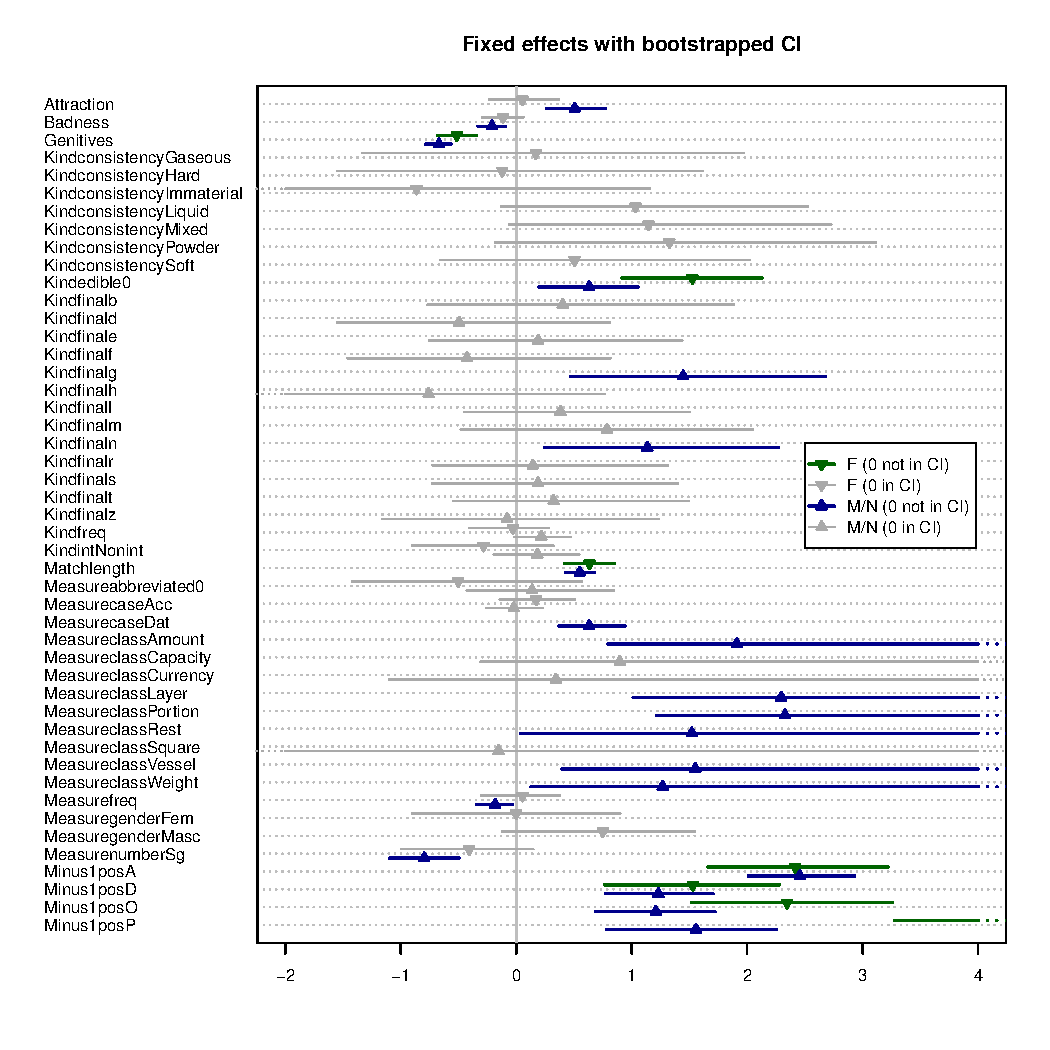
\includegraphics[width=0.9\textwidth]{figures/corpus/04_glmm_fixef.pdf}
\caption{Fixed effects in GLMMs for Masculine\slash Neuter and Feminine with 95\% bootstrapped confidence intervals (1,000 replicates)}
\label{fig:glmmfixef}
\end{figure}


\begin{figure}[h]
\centering
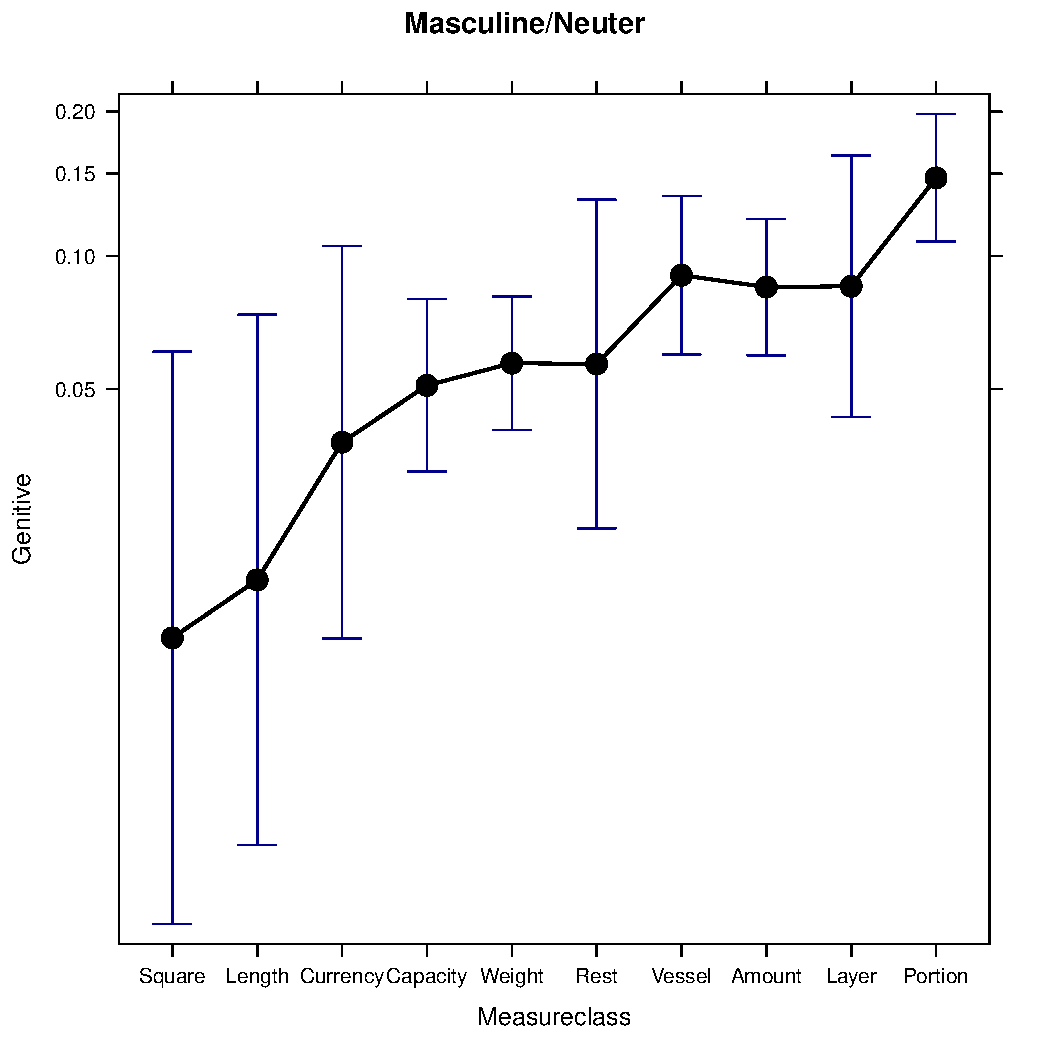
\includegraphics[width=0.6\textwidth]{figures/corpus/04_glmm_fixeff_mn_Measureclass}
\caption{Effect plot for the masculine\slash neuter GLMM: Measure lemma class effect}
\label{fig:glmm:fixef:measureclass}
\end{figure}

\begin{figure}[h]
\centering
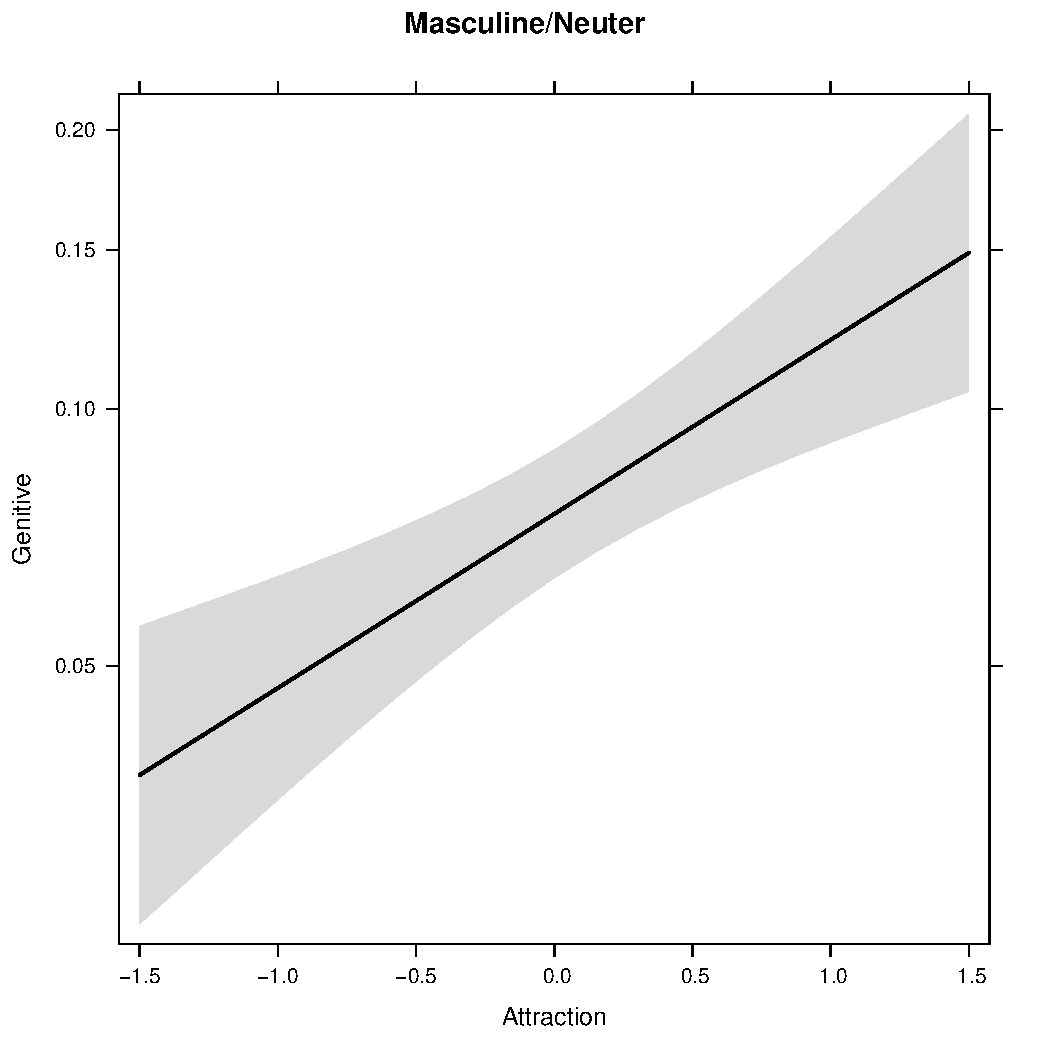
\includegraphics[width=0.4\textwidth]{figures/corpus/04_glmm_fixeff_mn_Attraction}~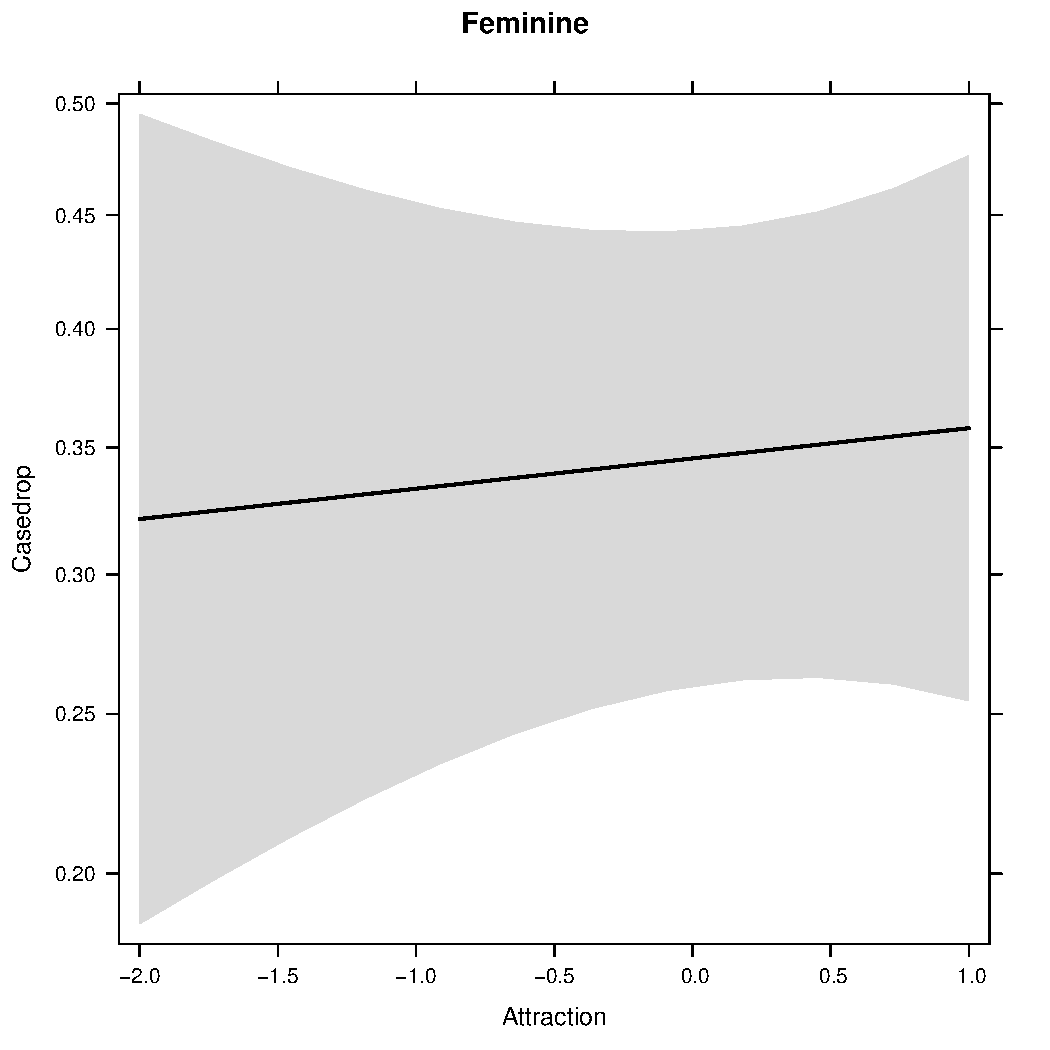
\includegraphics[width=0.4\textwidth]{figures/corpus/04_glmm_fixeff_fem_Attraction}
\caption{Effect plot for the two GLMMs: attraction effect (centered and standardised) from the NAC construction with a bare kind noun and the PGC with a determiner; scales are not aligned between left and right panel}
\label{fig:glmm:fixef:attraction}
\end{figure}

\begin{figure}[h]
\centering
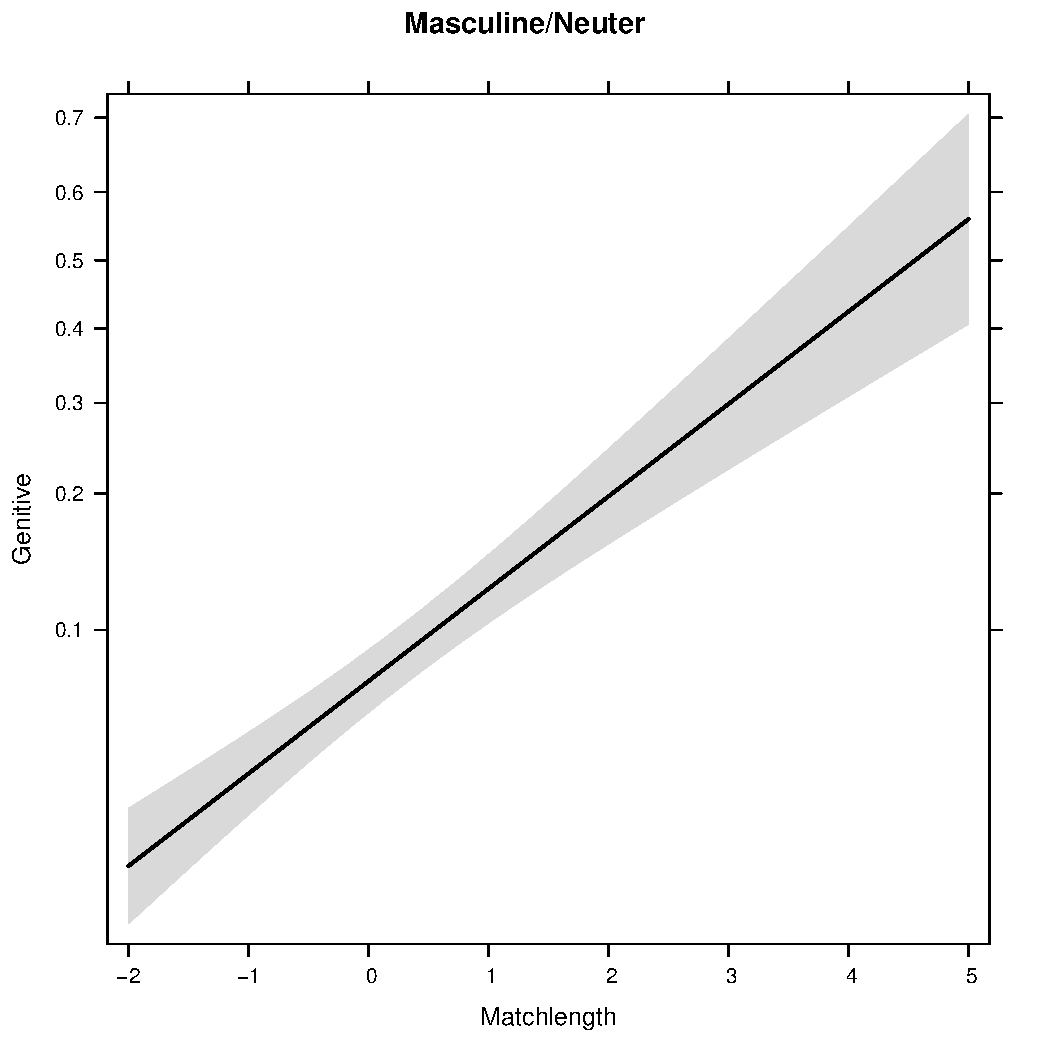
\includegraphics[width=0.4\textwidth]{figures/corpus/04_glmm_fixeff_mn_Matchlength}~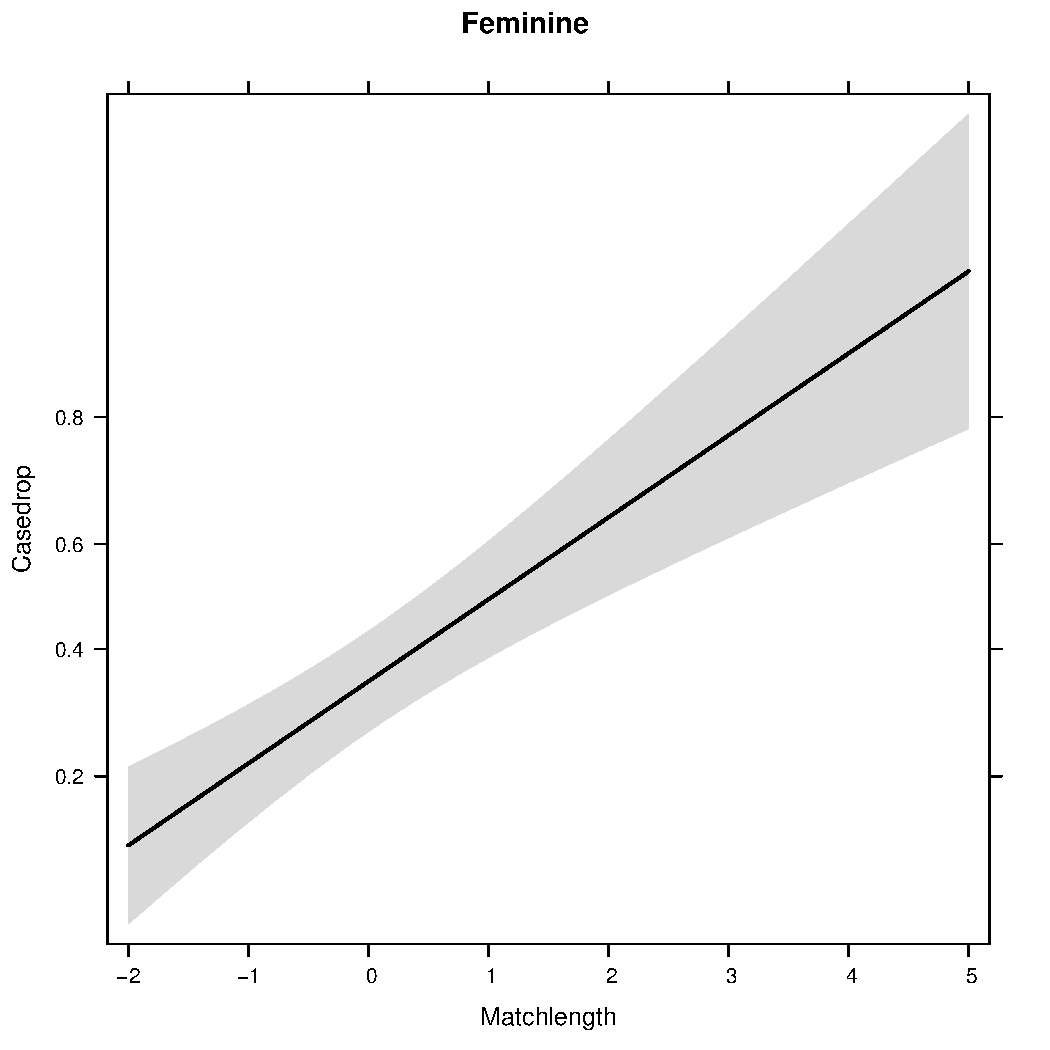
\includegraphics[width=0.4\textwidth]{figures/corpus/04_glmm_fixeff_fem_Matchlength}
\caption{Effect plot for the two GLMMs: effect of the (centered and standardised) length of the whole construction; scales are not aligned between left and right panel}
\label{fig:glmm:fixef:matchlength}
\end{figure}

\begin{figure}[h]
\centering
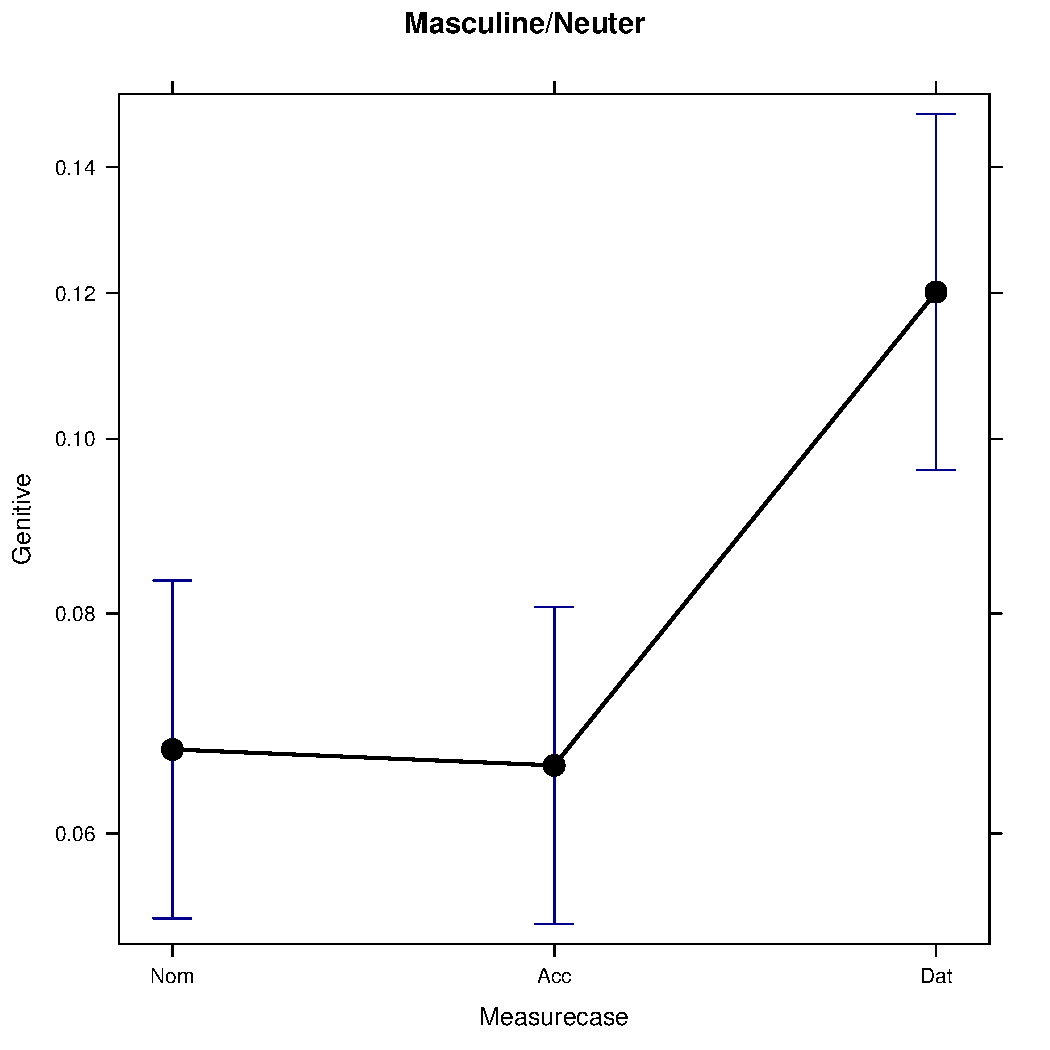
\includegraphics[width=0.4\textwidth]{figures/corpus/04_glmm_fixeff_mn_Measurecase}~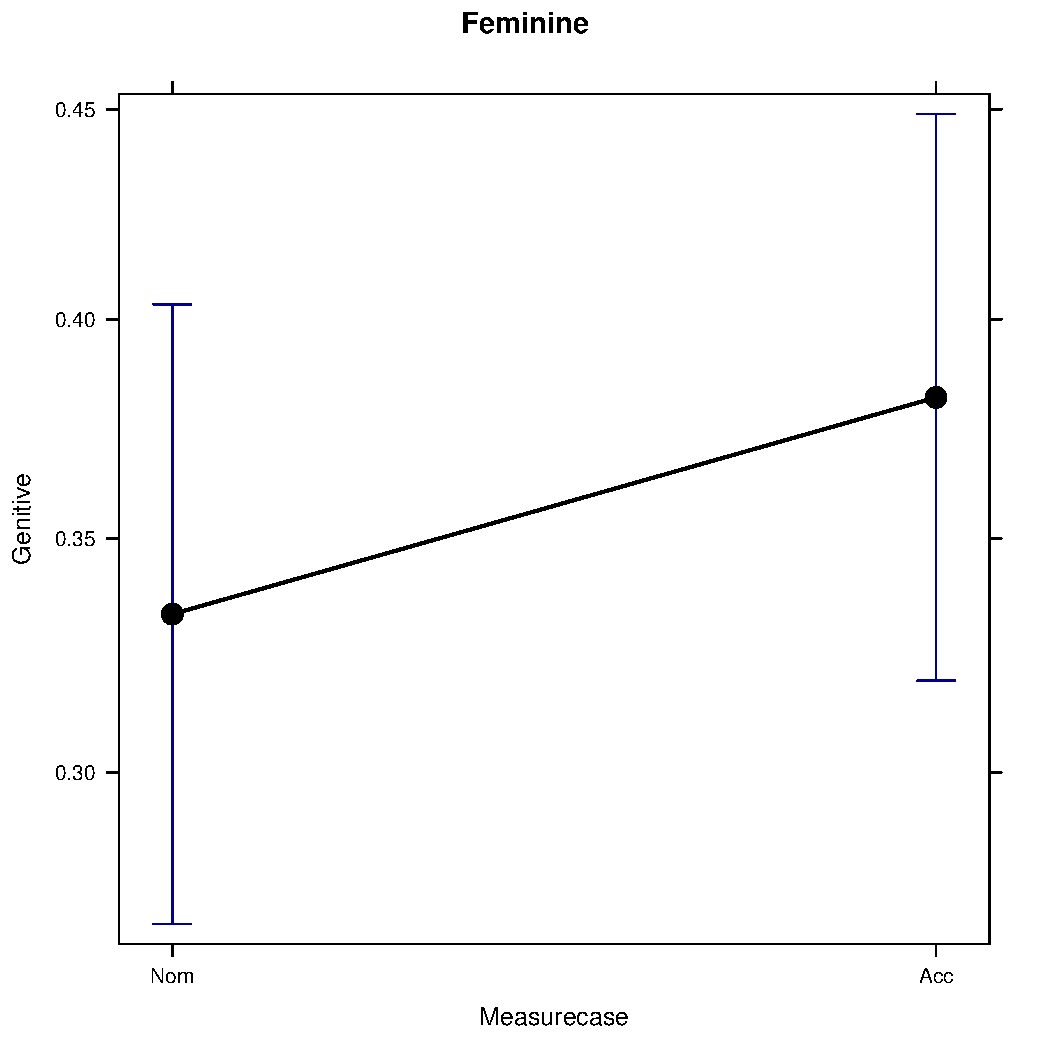
\includegraphics[width=0.4\textwidth]{figures/corpus/04_glmm_fixeff_fem_Measurecase}
\caption{Effect plot for the two GLMMs: effects of the case of the head (kind) noun; scales are not aligned between left and right panel}
\label{fig:glmm:fixef:measureclass}
\end{figure}

\begin{figure}[h]
\centering
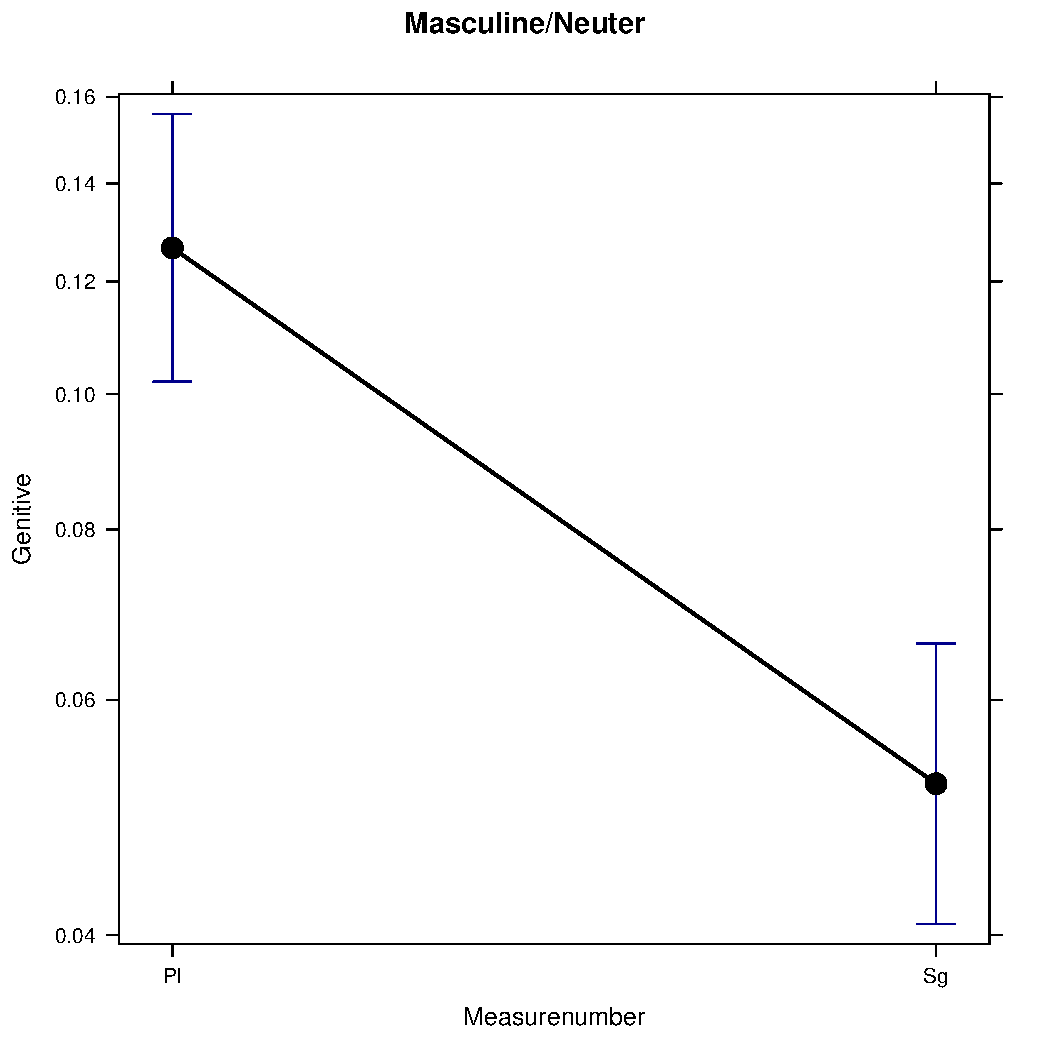
\includegraphics[width=0.4\textwidth]{figures/corpus/04_glmm_fixeff_mn_Measurenumber}~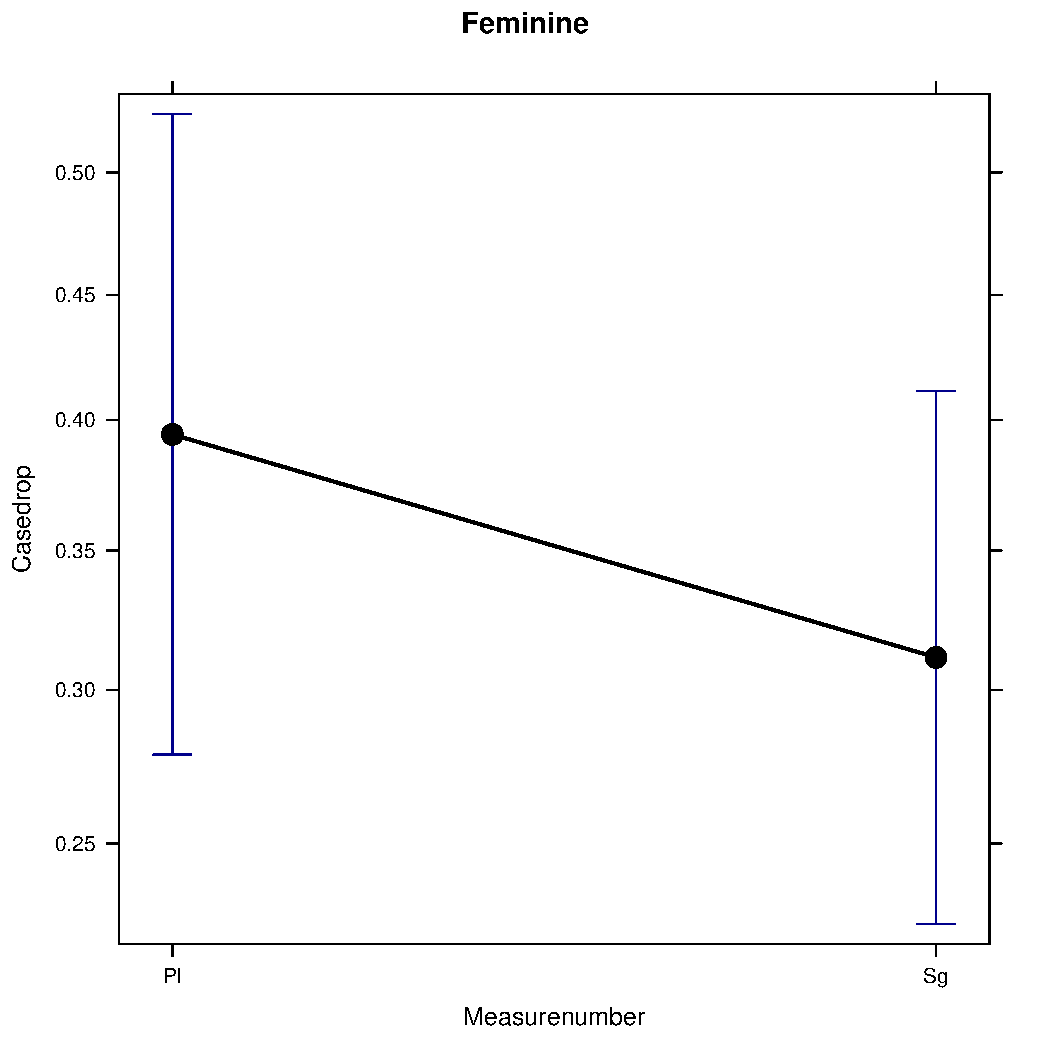
\includegraphics[width=0.4\textwidth]{figures/corpus/04_glmm_fixeff_fem_Measurenumber}
\caption{Effect plot for the two GLMMs: effect of the grammatical number of the head (kind) noun; scales are not aligned between left and right panel}
\label{fig:glmm:fixef:measurenumber}
\end{figure}

\begin{figure}[h]
\centering
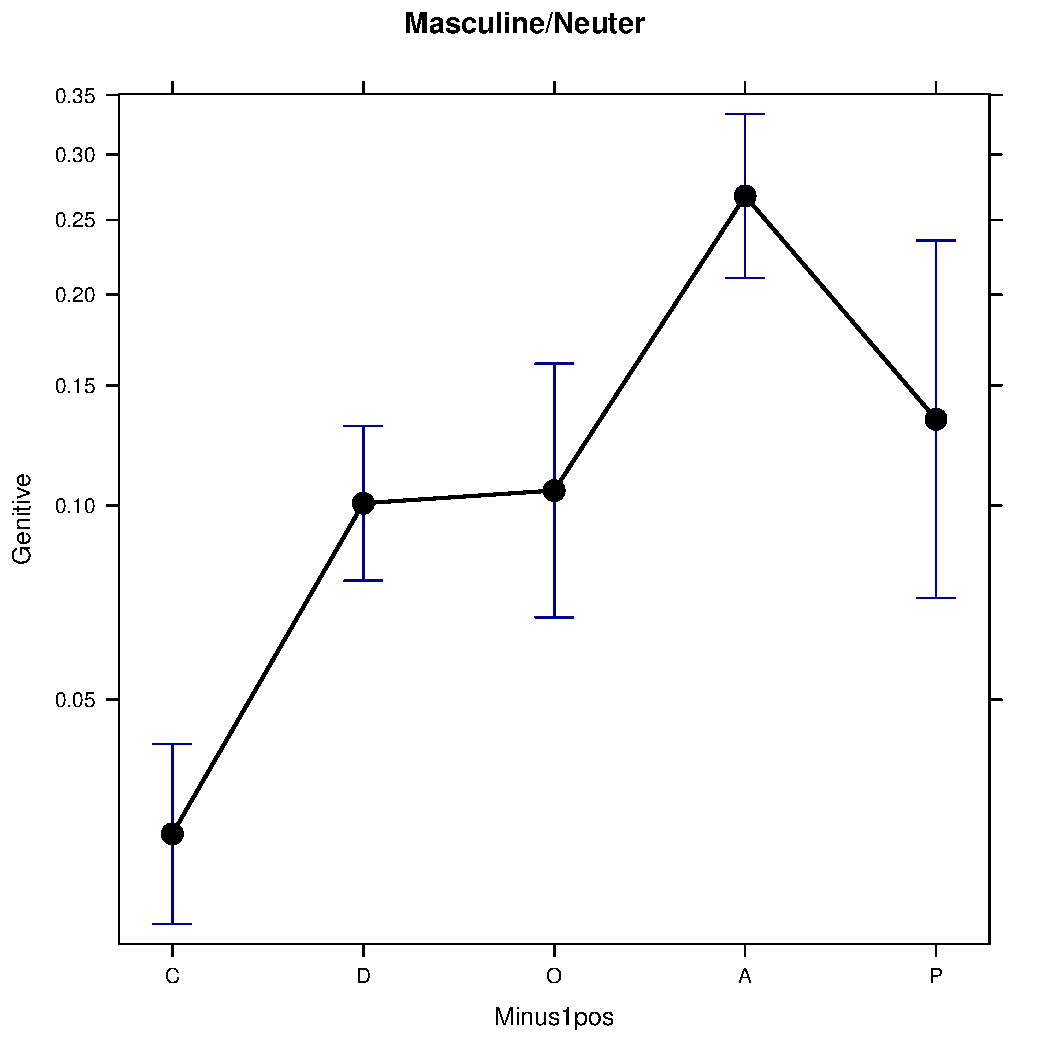
\includegraphics[width=0.4\textwidth]{figures/corpus/04_glmm_fixeff_mn_Minus1pos}~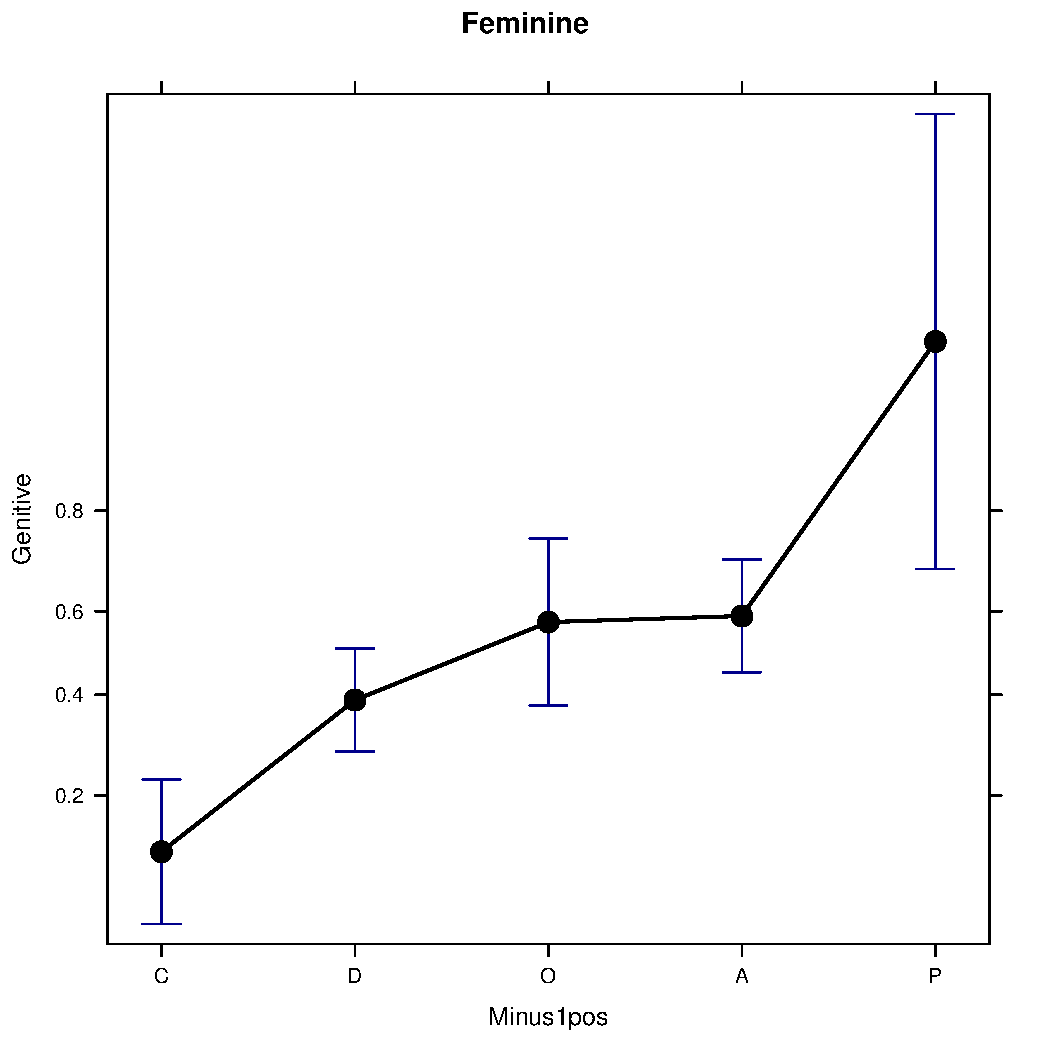
\includegraphics[width=0.4\textwidth]{figures/corpus/04_glmm_fixeff_fem_Minus1pos}
\caption{Effect plot for the two GLMMs: effect of part-of-speech preceding the construction; C = cardinal, D = determiner, O = \textit{other}, A = adjective, P = preposition; scales are not aligned between left and right panel}
\label{fig:glmm:fixef:minus1pos}
\end{figure}

\begin{figure}[h]
\centering
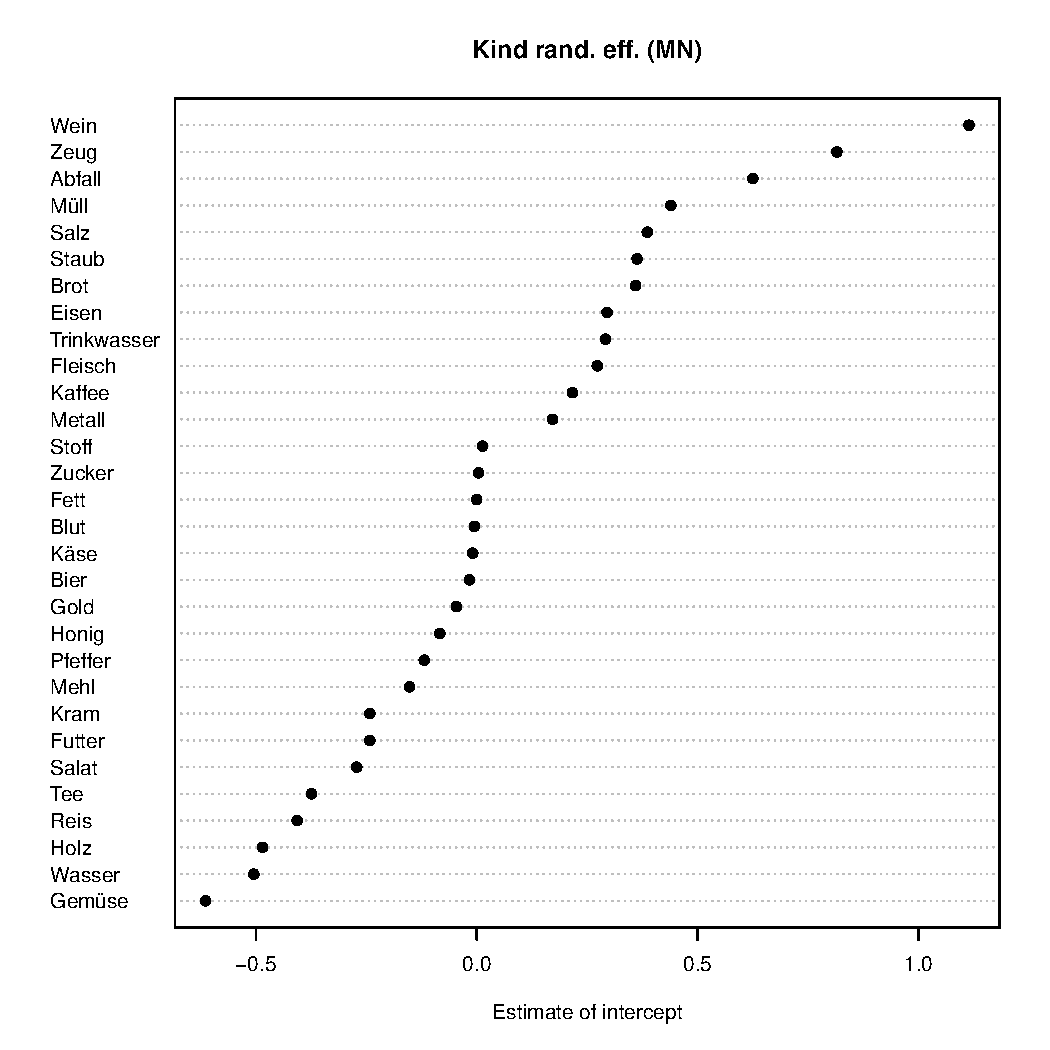
\includegraphics[width=0.5\textwidth]{figures/corpus/04_glmm_raneff_mn}~\hspace{0.05\textwidth}~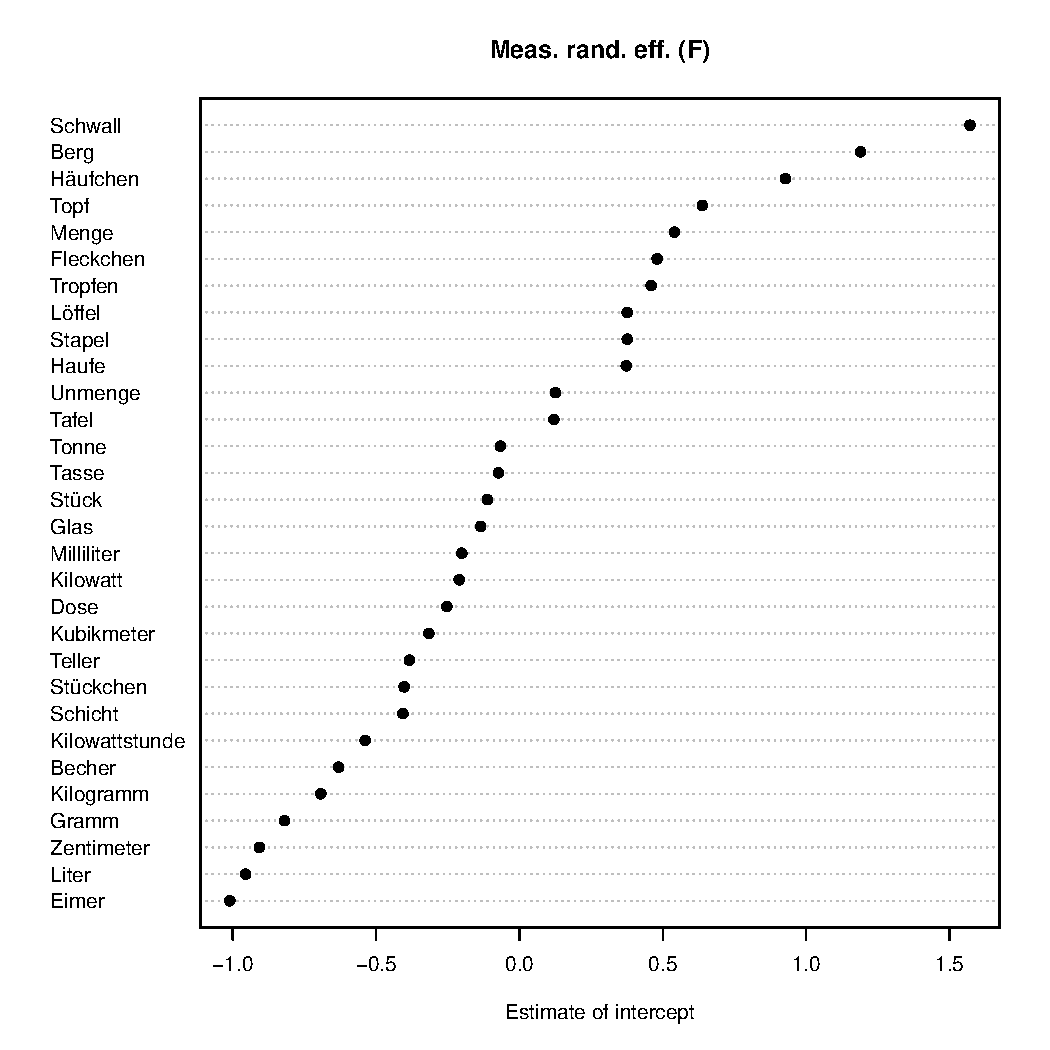
\includegraphics[width=0.5\textwidth]{figures/corpus/04_glmm_raneff_fem}
\caption{Sample random effects for the masculine\slash neuter and feminine GLMMs}
\label{fig:glmm:fixef:minus1pos}
\end{figure}




\subsection{A note on Bayesian estimation}
\label{ssec:bayesian}



\subsection{Summary and conclusions}
\label{ssec:modelssummary}

\begin{sidewaystable}
  \resizebox{1\linewidth}{!}{
  \begin{tabular}{lllp{2em}rrrrrcp{1em}rrrrcp{2em}rrrrrcp{1em}rrrrc}
         &                    &             && \multicolumn{12}{l}{Masculine\slash Neuter}                                                              && \multicolumn{12}{l}{Feminine}                                                                       \\
         &                    &             && \multicolumn{6}{l}{ML with Bootstrap Confidence Interval} && \multicolumn{5}{l}{MCMC}                    && \multicolumn{6}{l}{ML with Bootstrap Confidence Interval} && \multicolumn{5}{l}{MCMC}               \\
Level    & Regressor          & Value       && p(PB)  & Coef  & Low      & High  & Width  & Not 0        && Coef     & Low    & High  & Width   & Not 0 && p(PB)  & Coef  & Low   & High  & Width & Not 0            && Coef  & Low   & High  & Width &  Not 0 \\   \midrule

First    & Badness            & (numeric)   &&  0.002 &  -0.2 &    -0.32 & -0.08 &   0.24 &      †       &&     -0.2 &  -0.33 & -0.08 &    0.25 &     † &&  0.189 & -0.12 &  -0.3 &  0.08 &  0.37 &                  && -0.12 & -0.31 &  0.06 &  0.38 &        \\
         & Genitives          & (numeric)   &&  0.004 & -0.66 &    -0.77 & -0.54 &   0.23 &      †       &&    -0.67 &  -0.79 & -0.56 &    0.23 &     † &&  0.002 & -0.52 & -0.71 & -0.34 &  0.37 &     †            && -0.56 & -0.75 & -0.37 &  0.38 &      † \\

         & Matchlength        & (numeric)   &&  0.002 &  0.54 &      0.4 &  0.68 &   0.28 &      †       &&     0.59 &   0.45 &  0.73 &    0.27 &     † &&  0.002 &  0.63 &  0.41 &  0.86 &  0.45 &     †            &&  0.69 &  0.44 &  0.96 &  0.51 &      † \\
         & Measureabbreviated & 0           &&  0.730 &   0.1 &    -0.41 &  0.73 &   1.15 &              &&     0.07 &  -0.59 &  0.74 &    1.33 &       &&  0.267 & -0.65 & -1.67 &  0.41 &  2.08 &                  && -0.64 & -1.78 &   0.5 &  2.28 &        \\
         & Measurecase        & Acc         &&  0.002 & -0.02 &    -0.25 &  0.22 &   0.47 &              &&    -0.02 &  -0.25 &  0.23 &    0.48 &       &&  0.333 &  0.17 & -0.15 &  0.51 &  0.66 &                  &&  0.19 & -0.15 &  0.54 &   0.7 &        \\
         & Measurecase        & Dat         &&        &  0.63 &     0.35 &  0.92 &   0.57 &      †       &&     0.66 &   0.38 &  0.94 &    0.57 &     † &&        &       &       &       &       &                  &&       &       &       &       &        \\
         & Measurenumber      & Sg          &&  0.002 & -0.73 &    -1.03 & -0.42 &   0.61 &      †       &&    -0.72 &  -1.05 & -0.39 &    0.66 &     † &&  0.160 & -0.43 & -1.05 &  0.13 &  1.18 &                  && -0.39 & -0.97 &  0.17 &  1.14 &        \\
         & Minus1pos          & A           &&  0.002 &  2.45 &     1.97 &  2.89 &   0.92 &      †       &&     2.49 &   2.03 &  2.95 &    0.92 &     † &&  0.002 &  2.29 &  1.43 &  3.25 &  1.83 &     †            &&  2.17 &  1.36 &  2.98 &  1.63 &      † \\
         & Minus1pos          & D           &&        &  1.27 &     0.82 &  1.74 &   0.93 &      †       &&     1.23 &   0.76 &  1.69 &    0.93 &     † &&        &  1.48 &  0.64 &  2.33 &  1.69 &     †            &&  1.31 &  0.49 &  2.15 &  1.65 &      † \\
         & Minus1pos          & O           &&        &  1.32 &     0.82 &  1.82 &      1 &      †       &&     1.37 &   0.87 &  1.87 &    0.99 &     † &&        &  2.24 &  1.42 &   3.2 &  1.78 &     †            &&  2.14 &  1.24 &  3.02 &  1.77 &      † \\
	 & Minus1pos          & P           &&        &  1.59 &     0.87 &  2.27 &    1.4 &      †       &&     1.58 &   0.88 &  2.31 &    1.43 &     † &&        &  4.97 &  3.17 & 19.71 & 16.55 &     †            &&  4.67 &  2.93 &  6.68 &  3.75 &      † \\[\baselineskip]

Second   & Kindattraction     & (numeric)   &&  0.004 &  0.49 &     0.18 &  0.76 &   0.58 &      †       &&     0.51 &   0.19 &  0.82 &    0.63 &     † &&  0.855 &  0.03 & -0.26 &  0.32 &  0.58 &                  &&     0 & -0.42 &   0.4 &  0.82 &        \\
(kind    & Kindconsistency    & Gaseous     &&        &       &          &       &        &              &&          &        &       &         &       &&  0.070 &  0.15 & -1.29 &  1.78 &  3.08 &                  && -0.13 & -1.84 &  1.59 &  3.43 &        \\
lemma)   & Kindconsistency    & Hard        &&        &       &          &       &        &              &&          &        &       &         &       &&        & -0.23 & -1.65 &  1.42 &  3.07 &                  && -0.47 & -2.25 &  1.21 &  3.45 &        \\
         & Kindconsistency    & Immaterial  &&        &       &          &       &        &              &&          &        &       &         &       &&        & -1.03 & -2.49 &  0.67 &  3.15 &                  && -1.17 & -2.86 &  0.64 &  3.49 &        \\
         & Kindconsistency    & Liquid      &&        &       &          &       &        &              &&          &        &       &         &       &&        &  1.07 & -0.11 &  2.62 &  2.73 &                  &&     1 & -0.36 &  2.42 &  2.78 &        \\
         & Kindconsistency    & Mixed       &&        &       &          &       &        &              &&          &        &       &         &       &&        &     1 & -0.24 &  2.51 &  2.75 &                  &&  0.78 & -0.69 &  2.27 &  2.96 &        \\
         & Kindconsistency    & Powder      &&        &       &          &       &        &              &&          &        &       &         &       &&        &  1.18 & -0.41 &  3.01 &  3.42 &                  &&  1.01 & -0.88 &  2.84 &  3.72 &        \\
         & Kindconsistency    & Soft        &&        &       &          &       &        &              &&          &        &       &         &       &&        &   0.4 & -0.78 &  1.74 &  2.52 &                  &&  0.19 & -1.14 &  1.52 &  2.65 &        \\
         & Kindedible         & 0           &&  0.006 &  0.71 &     0.31 &  1.11 &   0.79 &      †       &&     0.71 &   0.26 &  1.17 &    0.91 &     † &&  0.006 &  1.44 &  0.76 &  2.03 &  1.27 &     †            &&  1.47 &  0.62 &  2.29 &  1.68 &      † \\
         & Kindfreq           & (numeric)   &&  0.585 &  0.08 &     -0.2 &  0.34 &   0.54 &              &&     0.09 &   -0.2 &  0.37 &    0.57 &       &&  0.979 & -0.01 & -0.36 &  0.33 &  0.69 &                  &&  0.03 & -0.45 &  0.51 &  0.96 &        \\
         & Kindint            & Nonint      &&  0.432 &  0.16 &    -0.24 &  0.54 &   0.78 &              &&     0.18 &  -0.27 &  0.65 &    0.92 &       &&  0.326 &  -0.3 & -0.88 &  0.32 &   1.2 &                  && -0.18 & -0.94 &   0.7 &  1.64 &        \\[\baselineskip]

Second   & Measureattraction  & (numeric)   &&  0.033 &  0.21 &     0.06 &  0.36 &    0.3 &      †       &&     0.22 &  -0.01 &  0.46 &    0.47 &       &&  0.006 &  0.43 &  0.09 &  0.75 &  0.66 &     †            &&  0.54 &  0.18 &  0.96 &  0.78 &      † \\
(measure & Measureclass       & Amount      &&  0.004 &  1.97 &     0.76 & 16.34 &  15.58 &      †       &&     1.43 &   0.26 &  2.75 &    2.49 &     † &&        &       &       &       &       &                  &&       &       &       &       &        \\
lemma)   & Measureclass       & Capacity    &&        &  1.42 &     0.09 & 15.78 &  15.69 &      †       &&     0.67 &  -0.62 &  1.96 &    2.57 &       &&        &       &       &       &       &                  &&       &       &       &       &        \\
         & Measureclass       & Currency    &&        &   1.1 &    -0.59 & 15.65 &  16.24 &              &&     0.34 &  -1.21 &  1.93 &    3.14 &       &&        &       &       &       &       &                  &&       &       &       &       &        \\
         & Measureclass       & Layer       &&        &  1.98 &      0.6 & 16.42 &  15.81 &      †       &&     1.33 &  -0.09 &  2.85 &    2.95 &       &&        &       &       &       &       &                  &&       &       &       &       &        \\
         & Measureclass       & Length      &&        &  0.33 &   -13.69 & 14.69 &  28.37 &              &&    -0.52 &  -2.55 &  1.26 &    3.81 &       &&        &       &       &       &       &                  &&       &       &       &       &        \\
         & Measureclass       & Portion     &&        &  2.58 &     1.38 & 17.01 &  15.63 &      †       &&     1.97 &   0.85 &  3.18 &    2.33 &     † &&        &       &       &       &       &                  &&       &       &       &       &        \\
         & Measureclass       & Rest        &&        &  1.54 &    -0.14 & 15.95 &  16.09 &              &&     0.79 &  -0.71 &  2.24 &    2.95 &       &&        &       &       &       &       &                  &&       &       &       &       &        \\
         & Measureclass       & Vessel      &&        &  2.04 &     0.76 & 16.44 &  15.69 &      †       &&     1.43 &   0.22 &  2.69 &    2.47 &     † &&        &       &       &       &       &                  &&       &       &       &       &        \\
         & Measureclass       & Weight      &&        &  1.54 &     0.35 & 15.95 &   15.6 &      †       &&     1.07 &  -0.14 &  2.43 &    2.57 &       &&        &       &       &       &       &                  &&       &       &       &       &        \\
         & Measurefreq        & (numeric)   &&  0.041 & -0.16 &    -0.31 & -0.02 &    0.3 &      †       &&    -0.17 &  -0.37 &  0.04 &    0.41 &       &&  1.000 &     0 & -0.34 &  0.34 &  0.68 &                  &&  0.03 & -0.37 &  0.49 &  0.86 &        \\
  \end{tabular}
  }
  \smallskip
  \caption{Coefficients with confidence intervals from GLMMs with Maximum Likelihood and MCMC estimation}
  \label{tab:bigtable}
\end{sidewaystable}





\section{Experimental cross-check of the corpus-based models}
\label{sec:externalvalidation}

% TODO SURPRISAL
%
% Bybee, Joan und Thompson, Sandra. 1997. “Three Frequency Effects in Syntax”, Proceedings of the Twenty-Third Annual Meeting of the Berkeley Linguistics Society, 378-388.
% Bybee, Joan. 2006. “From Usage to Grammar: The Mind‘s Response to Repetition”. Language 82(4): 711-733.
% Levy, Roger .2008. “Expectation-based syntactic comprehension.” Cognition 106: 1126–1177.
% Smith, Nathaniel, and Levy, Roger. 2013. “The effect of word predictability on reading time is logarithmic.” Cognition 128: 302–319.

\subsection{Experiment 1: forced choice}

As was pointed out in Section \ref{ssec:cocl}, there can be substantial doubt that corpus linguistic methods in themselves can be called \textit{cognitively oriented} in any meaningful way.
At the same time, it is a highly plausible assumption in a usage-based framework that large and varied corpora ideally represent language users' relevant input of (at least) written language, and that there should be reflexes of the distributions found in such corpora in the linguistic behaviour of language users.
Therefore, this section and the next present the results of two experiments wherein I cross-checked the corpus-based findings.

First, a very simple computer-aided forced-choice experiment was conducted.%
\footnote{The experiment is \textit{simple} compared to the sophisticated origins of forced choice experiments and their interpretation in psychophysics \citep[166--179]{MacmillanCreelman2005}.}
From a linguistic point of view, the forced choice setting has the advantage over rating studies that is does not force participants into making an absolute acceptability judgement on some scale.
Instead, they express a preference for one of two constructions (or words, etc.) both of which are acceptable.
While this does not totally exclude normative thinking -- to which native speakers of German in so-called \textit{cases of doubt} are typically prone -- 

There were 24 participants aged 19 to 30 who were recruited from introductory linguistics courses at Freie Universität Berlin.
Although the experiment was conducted in the last four weeks of their first semester, participants had no deeper explicit knowledge of linguistics or grammar.%
\footnote{Even though the ratio of target sentences to fillers was relatively high (see below) and some of the fillers were also related to case alternations, no participant used the word \textit{Kasus} `case' when asked whether they had an idea what the experiment was about in informal interviews after the experiment.}
Only participants with an L1 background in German were recruited.

As stimuli, I used attested (but simplified) sentences from the corpus study in an approach similar to the one taken in \cite{DivjakEa2016}.
The rationale was that it is virtually impossible to test the large and complex sets of regressors used in the corpus study in a traditional randomized experiments where usually just one relevant factor (ideally something like treatment vs.\ non-treatment) is of interest.
Therefore, attested sentences were used, and the predictions of the corpus models were tested against participants' preferences.

Concretely, I sampled 16 attested sentences from the corpus and simplified them (mostly removing embedded clauses, complex adverbials, etc.) and standardized their orthography.
It was made sure that the simplifications and normalisations did not affect any of the regressors used in the corpus study, of course.
Eight sentences contained masculine or neuter kind nouns, the other eight contained feminine kind nouns.
Furthermore, in each of the M\slash N and F groups, four sentences with a case drop (\ie\ genitive or oblique case on the kind noun) and four withe case identity were chosen.
More precisely, the four sentences were sampled as highly prototypical examples of case drop (high logits) and case identity (low logits), respectively, according to the corpus based models.%
\footnote{Sentences were sorted by their corresponding $\hat{y}$ calculated from the model.
For the M\slash N sentences, sentences were sampled from the top and bottom 15\% of the resulting vector.
For the F sentences, the top and bottom 25\% were used because the overall sample size was smaller.}
It was made sure that the highly predictive features according to Section \ref{ssec:modelssummary} occurred in unique combinations among the four sentences in each cell.
This is summarised in Table \ref{tab:experiment1:design}.

\begin{table}
  \centering
  \begin{tabular}[h]{rcc}
     & M\slash N & F \\
     \midrule
     \textbf{high prob.\ for case drop} & 4 sentences\Supsf{a} & 4 sentences\Supsf{a} \\
     \textbf{low prob.\ for case drop} & 4 sentences\Supsf{a} & 4 sentences\Supsf{a} \\
  \end{tabular}
  \caption{The four groups of attested sentences chosen as stimuli (\Supsf{a}Among the 4 sentences, combinations of important factor values were made unique.)}
  \label{tab:experiment1:design}
\end{table}

The pairs of stimuli were the original attested sentence containing the preferred construction and a modified version containing the dispreferred construction.
They were presented next to each other, and a 20 second time limit for each choice was set.%
\footnote{No participant ever exceeded the time limit.}
The position on the screen (left\slash right) and the order of sentences were randomized for each participant.
As fillers, 23 pairs of sentences exemplifying similar alternation phenomena from German morpho-syntax were used.
Thus, participants saw 39 pairs of sentences and 78 sentences in total.
They were instructed to select from each pair of sentences the one that seemed more natural to them in the sense that they would use it rather than the other one.
The experiment was conducted using \textit{PsychoPy} \citep{Peirce2007}.

\begin{figure}[h]
\centering
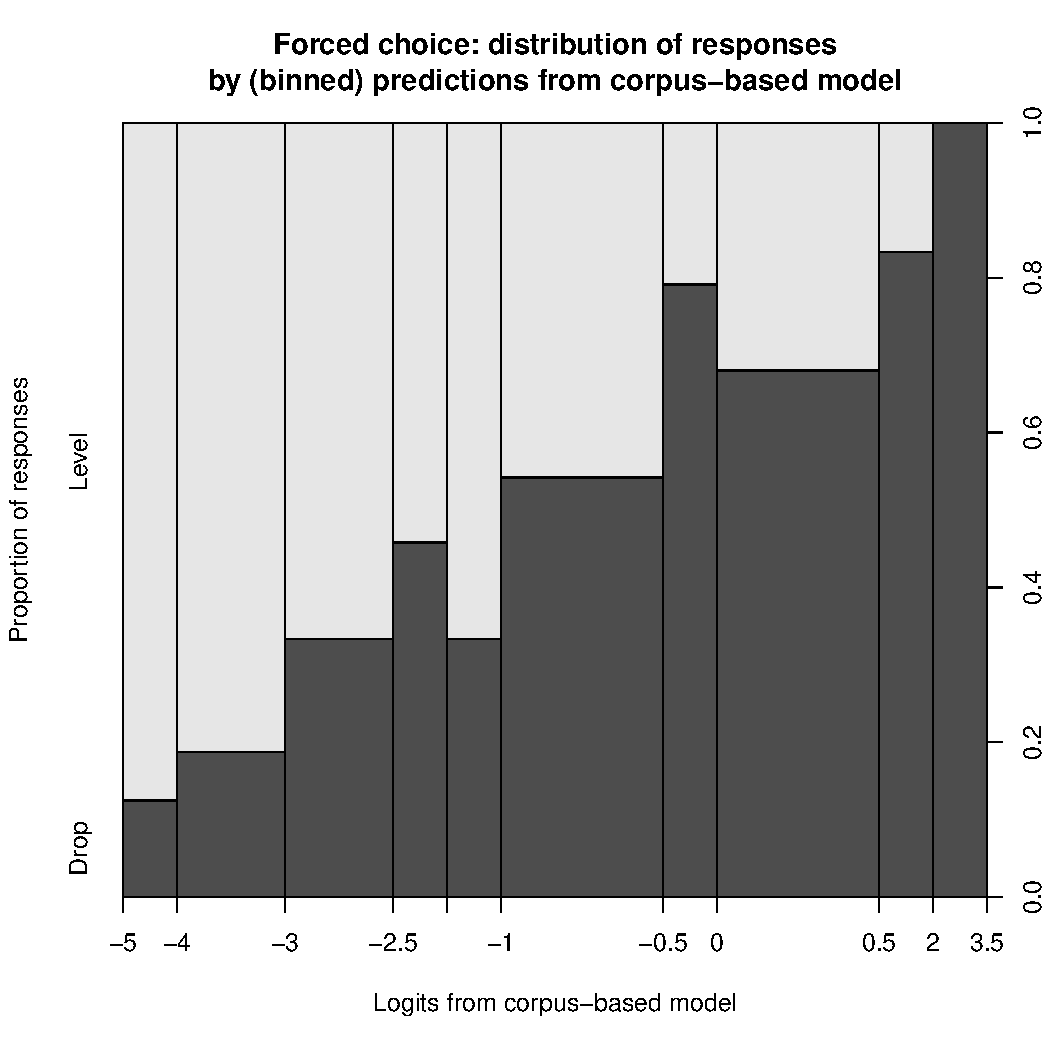
\includegraphics[width=0.6\textwidth]{figures/experiment/2afc_proportions}
\caption{Participants' responses in the forced-choice task plotted against the predictions from the corpus-based model}
\label{fig:afc:proportions}
\end{figure}

Descriptively, Figure \ref{fig:afc:proportions} shows the relationship between the logits calculated from the corpus-based model and the proportional choices made by participants.
Visually, it looks like there is a close correlation between the corpus-derived preferences and preferences in the forced choice experiment.

Then, a multilevel logistic regression was specified as in Equation \ref{eq:model:afc}.

\begin{equation}
  \begin{split}
  Pr(y_i=1) & = logit^{-1}(\beta^0+\beta^1\cdot x_i^1+\beta^2\cdot x_i^2+\beta^{1.2}\cdot x_i^1\cdot x_i^2+ \\
  & + \alpha^{\text{Item}}_{j_i} + \alpha^{\text{Participant}}_{k_i}) \\
  \text{where}\ \ & x^1 = \text{\it Modelpred} \\
  & x^2 = \text{\it KindgenderMN} \\
  %ResponseDrop~Modelpred*Kindgender+(1|Item)+(1|Participant)
  \end{split}
  \label{eq:model:afc}
\end{equation}

Coefficients were estimated using Maximum Likelihood, and the coefficient table is given in Table \ref{tab:afc:model}, where instead of approximate standard errors and $z$ and $p$ values the lower and the upper bound of a bootstrapped 95\% confidence interval are specified.

\begin{table}
  \centering
  \begin{tabular}{lrrr}
    Effect & Estimate & 95\% CI lower & 95\% CI upper \\
    \midrule
    (Intercept)            &  0.748  &  0.242  &  1.265 \\
    Modelpred              &  1.154  &  0.905  &  1.497 \\
    KindgenderMN           &  0.135  & -0.416  &  0.632 \\
    Modelpred:KindgenderMN & -0.567  & -0.843  & -0.298 \\
  \end{tabular}
  \caption{Coefficient table for the GLMM specified in equation \ref{eq:model:afc}, analysing the results of the forced choice experiment}
  \label{tab:afc:model}
\end{table}

The number of observations was $n=768$.
The random effects for participant ($\sigma=0.7841$, 24 groups) and item ($\sigma=0.4869$, 16 groups) show considerable variance.
Accordingly, there is a notable difference between the marginal and conditional Nakagawa \& Schielzeth's $R^2_{m}=0.383$ and $R^2_{c}=0.510$, while both values are quite high.
Dropping the term of interest ($\beta^1\cdot x_i^1+\beta^2\cdot x_i^2+\beta^{1.2}\cdot x_i^1\cdot x_i^2$) leads to a significantly worse fit of the nested model both in a traditional Likelihood Ratio Test ($LR=55.172$, $p<0.0001$) and its bootstrapped PB alternative ($p = 0.002$, 493 of 500 requested samples used).
The effect display for the term is given in Figure \ref{fig:afc:effects}.

\begin{figure}[h]
\centering
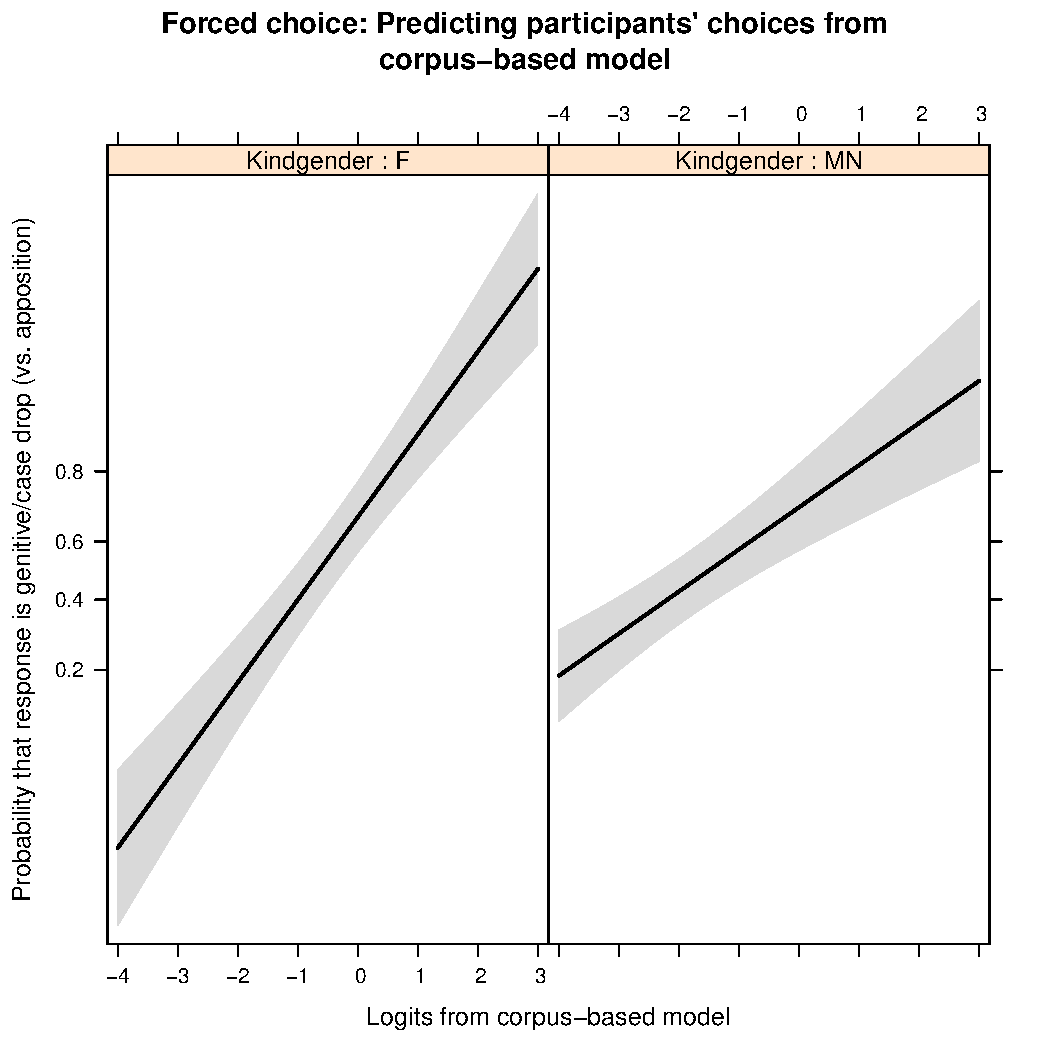
\includegraphics[width=0.6\textwidth]{figures/experiment/2afc_effects}
\caption{Effect plot for the multilevel logistic regression in the forced-choice experiment: predictability of participants' choices from the logits of the corpus-based GLMM (cf.\ Section~\ref{ssec:corpushierarchicalmodel})}
\label{fig:afc:effects}
\end{figure}

In summary, the forced choice experiment clearly succeeded in validating the results from the corpus study in as much as the preferences extracted from the corpus correspond to native speakers' choices.
We can take this as an indication that there is some relation between the process generating the corpus data and the behaviour of individual speakers.
In the next section, I report the results of a self-paced reading experiment which yielded (maybe expectedly) less clear results.


\subsection{Experiment 2: self-paced reading}


%\begin{figure}[h]
%\centering
%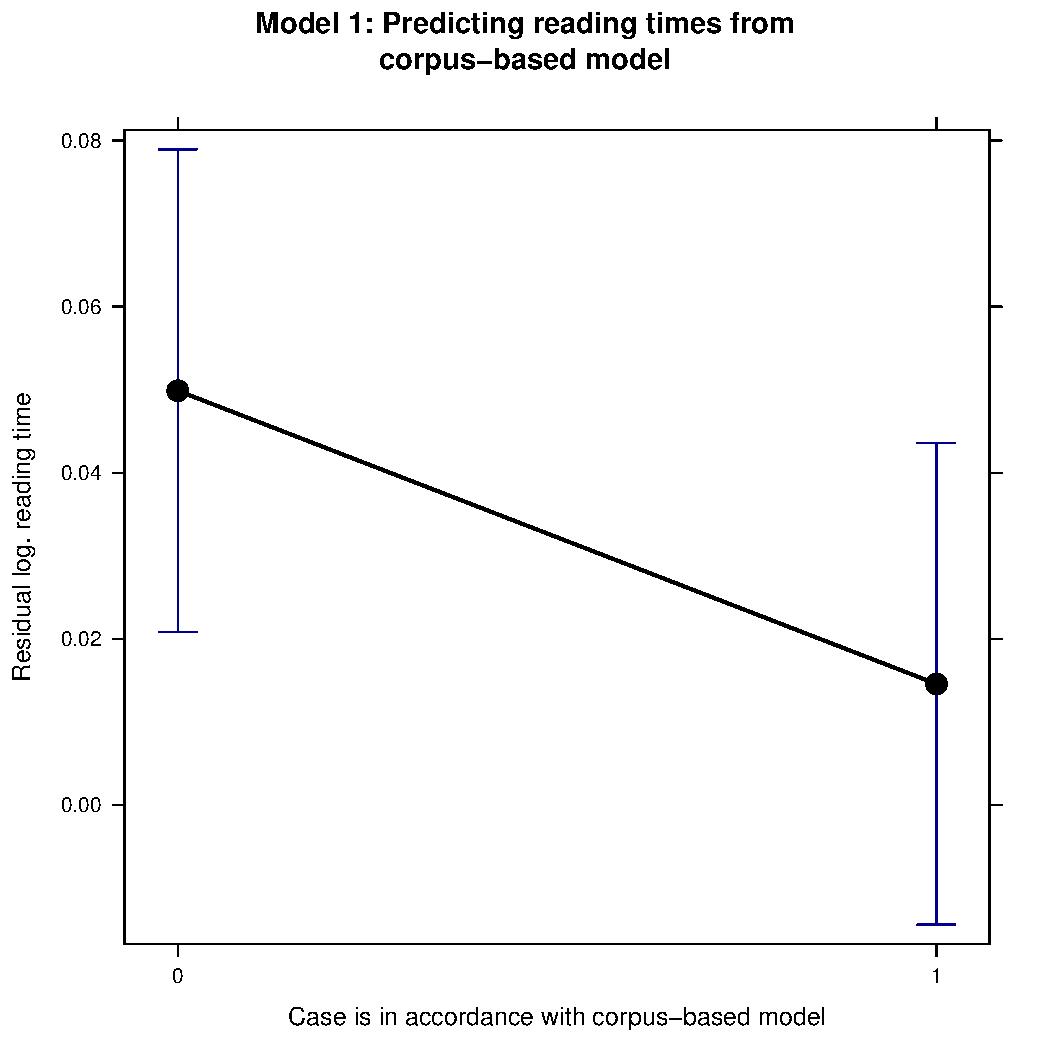
\includegraphics[width=0.6\textwidth]{figures/experiment/spr_effects_modelPredDichotomousReg}
%\caption{Effect plot for the LMM in the self-paced reading experiment: modeling participants' residualised log reading times on the dichotomised predictions of the corpus-based GLMM (cf.\ Section~\ref{ssec:corpushierarchicalmodel})}
%\label{fig:spr:dichotomous:effects}
%\end{figure}

\begin{figure}[h]
\centering
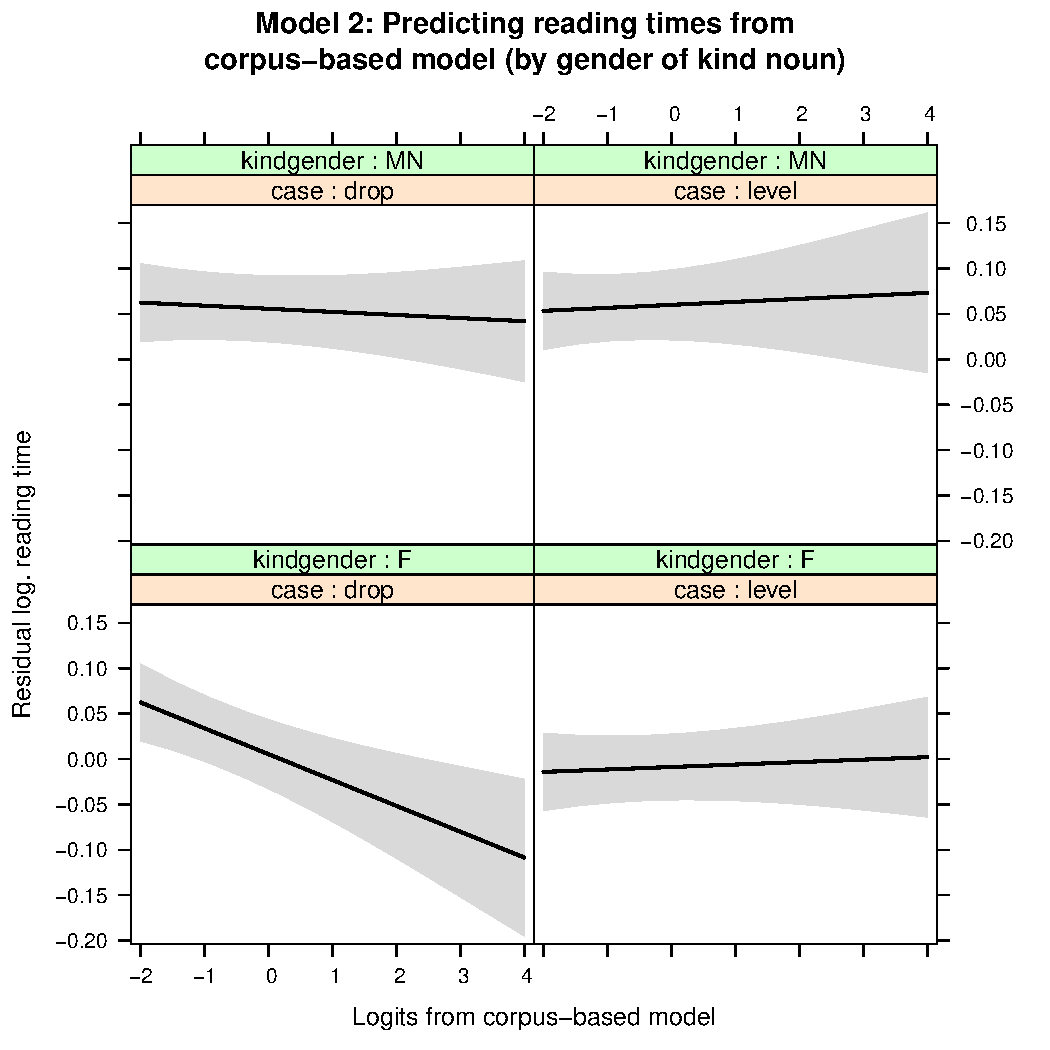
\includegraphics[width=0.6\textwidth]{figures/experiment/spr_effects_case+modelPred+gender}
\caption{Effect plot for the LMM in the self-paced reading experiment: modeling participants' residualised log reading times on the predictions (logits) of the corpus-based GLMM (cf.\ Section~\ref{ssec:corpushierarchicalmodel})}
\label{fig:spr:continuous:effects}
\end{figure}



\section{Conclusions}




\begin{acknowledgement}
  I want to thank (in alphabetical order) Felix Bildhauer, Götz Keydana, and Ulrike Sayatz for stimulating discussions on relevant aspects of this paper.
  I also thank Ulrike Sayatz for recruiting the participants for the experiments.
  I am grateful to Kim Maser for her work on the annotation of the concordances.
  Furthermore, Samuel Reichert substantially helped to develop the guiding ideas behind this study by writing an excellent BA theses on the subject under my supervision.
  The research presented here was made possible in part through funding from the \textit{Deutsche Forschungsgemeinschaft} (DFG, personal grant SCHA1916/1-1).
\end{acknowledgement}


\bibliography{rs,cow}
\end{document}
